\documentclass[dutch,a4paper,12pt,doubleside]{book}

\usepackage[T1]{fontenc}
\usepackage[dutch]{babel}
\usepackage[utf8]{inputenc}
\usepackage[margin=3cm]{geometry}
\usepackage{amsthm}
\usepackage{hyperref}
\usepackage{minted}
\usepackage{float}
\usepackage{trimspaces}
\usepackage[nottoc]{tocbibind}
\usepackage[labelfont=bf]{caption}
\usepackage{tabularx}
\usepackage{array}
\usepackage{dirtree}

% headers and footers (page numbering)
\usepackage{fancyhdr}
\fancyhf{} % clear all header and footers
\renewcommand{\headrulewidth}{0pt} % remove the header rule
\fancyfoot[R]{\thepage} % Left side on Even pages; Right side on Odd pages
\pagestyle{fancy}
\fancypagestyle{plain}{%
  \fancyhf{}%
  \renewcommand{\headrulewidth}{0pt}%
  \fancyhf[lef,rof]{\thepage}%
}

% Card suits
\DeclareSymbolFont{extraup}{U}{zavm}{m}{n}
\DeclareMathSymbol{\varheart}{\mathalpha}{extraup}{86}
\DeclareMathSymbol{\vardiamond}{\mathalpha}{extraup}{87}

\usepackage{makeidx}
\usepackage{hyperref}
\usepackage{minted}

% New line per paragraph, instead of indentation
\usepackage[parfill]{parskip}

% Prevent balancing vertical alignment
\raggedbottom

% Sets global font
\usepackage{tgpagella}

% Font utility function
\newcommand{\fon}[1]{\fontfamily{#1}\selectfont}

\usepackage[table, x11names]{xcolor}
\definecolor{blue}{RGB}{0, 149, 200}
\definecolor{green}{RGB}{0, 200, 136}

\captionsetup{justification=raggedright,width=.8\linewidth}

\usepackage[many]{tcolorbox}
\newtcolorbox{deftbox}{
    enhanced,
    sharp corners,
    frame hidden,
    boxrule=0em,
    left=1em,
    toptitle=1em,
    top=0.25em,
    bottom=1em,
    bottomtitle=0mm,
    colback=black!4,
    colbacktitle=black!4,
    coltitle=black!60,
    fonttitle=\bfseries\small,
    fontupper=\small,
    borderline west={2pt}{0pt}{black!20},
    grow to left by=-2em,
    grow to right by=-2em
}
\newtcolorbox{defbox}[1]{
    enhanced,
    sharp corners,
    frame hidden,
    boxrule=0em,
    left=1em,
    toptitle=1em,
    top=0.25em,
    bottom=1em,
    bottomtitle=0mm,
    colback=black!4,
    colbacktitle=black!4,
    coltitle=black!60,
    fonttitle=\bfseries\small,
    fontupper=\small,
    borderline west={2pt}{0pt}{black!20},
    grow to left by=-2em,
    grow to right by=-2em,
    title={#1}
}
\newtcolorbox{quotebox}{
    enhanced,
    sharp corners,
    frame hidden,
    left=1em,
    right=1em,
    top=1em,
    bottom=1em,
    colback=black!4!white,
    fontupper=\small,
    grow to left by=-2em,
    grow to right by=-2em
}

\def\trim#1{\ignorespaces#1\unskip}

\newcommand{\blockquote}[2]{
    \hfill
    \begin{quotebox}
    \begin{flushleft}
        ``\trim{#1}''
        \newline\newline\rightline{\textbf{-- \trim{#2}}}
    \end{flushleft}
    \end{quotebox}
    \noindent
}

\renewcommand{\listingscaption}{Codevoorbeeld}
\renewcommand{\listoflistingscaption}{Overzicht van codevoorbeelden}
\counterwithin{listing}{chapter}
% \usepackage[chapter]{minted}



\hypersetup{
  colorlinks,
  allcolors=[rgb]{0.3,0.3,0.8},
  linktoc=all
}

\title{BEP2 Opdracht}
\author{A. Rothuis}

\begin{document}

% \part{De opdracht}
\chapter{Opdrachtbeschrijving}

De eindopdracht van deze cursus bestaat uit een Java-project met een mondeling assessment.

HU-land Casino is een aanbieder van online kansspelen. 
Spelers kunnen met speelgeld (\textit{chips}) hun favoriete spelletjes spelen. 
Mogelijk dat HU-land Casino in de toekomst een betaalde variant op de markt wil zetten, 
maar voor nu wil het bedrijf naamsbekendheid verwerven, advertenties aanbieden en ervaring opdoen. 

Voor hun spelletjessite wil HU-land Casino een variant van het bekende \textit{blackjack} aanbieden. 
Het deel om in te loggen is overgenomen van een bestaande component (\textit{security}). 
Ook is er al enige functionaliteit om chips toe te voegen wanneer de speler deze niet meer heeft. 
Omdat nog onduidelijk is op welke technologieën wordt ingezet en met welke andere systemen gecommuniceerd zal worden, 
is het van groot belang dat deze backend onderhoudbaar en flexibel wordt opgezet. 
Het bedrijf heeft al een aantal Java-applicaties draaien met behulp van het Spring Boot framework. 
Daarom is gekozen om ook deze applicatie met Java en Spring Boot op te zetten. 
HU-land Casino heeft aangegeven waarde te hechten aan standardisatie. 
Daarom is gevraagd extra aandacht te besteden aan object oriëntatie, design principles, design patterns en REST-principes.

Er is gekozen voor een back-end applicatie om centrale controle 
te houden op het spel, terwijl met HTTP en REST compatibiliteit wordt 
geboden met verschillende front-ends, 
waaronder desktop, mobile en web apps.

Aan jou de taak om jouw ontwerp- en programmeervaardigheden in te zetten om 
een losgekoppelde, maar geïntegreerde, backend API voor het blackjackspel aan te bieden!

\newpage

\section{Het spel}
Blackjack is het bekendste kaartspel dat in casino's te vinden is.
Het spel wordt gespeeld met 1 of meer decks met 52 standaard speelkaarten.

Elke speelkaart vertegenwoordigt een bepaalde waarde gebaseerd 
op de rang (\textit{rank}) die op de kaart staat. 
De kleur (\textit{suit}) is niet van belang voor de regels 
van het spel, maar natuurlijk wel voor het weergeven van het spel.

De speler probeert de dealer te verslaan door met de score van de kaarten 
in de hand dichter bij de 21 te komen dan de dealer, 
zonder boven de 21 uit te komen.

In onze variant is er sprake van 1-speler-blackjack. Er kunnen wel 
meerdere potjes tegelijk gespeeld worden door verschillende en dezelfde 
speler. Spelers mogen niet aan elkaars spel meedoen.

\subsection{Het spelverloop}
Laten we het spelverloop van blackjack bestuderen.
Let wel\: voor een web-applicatie kan het zijn dat sommige stappen
anders kunnen verlopen, bijvoorbeeld ten behoeve van de onderhoudbaarheid
of efficiëntie. Sommige stappen worden immers volledig geautomatiseerd. 
Om dezelfde reden kunnen sommige stappen worden samengevoegd. 
Op die manier beperken we bijvoorbeeld ook de hoeveelheid netwerkcommunicatie.

Het algemene spelverloop is als volgt:
\begin{enumerate}
    \item \textit{Start game}: de speler start het spel door chips in te zetten (\textit{bet})
    \item \textit{Shuffle deck}: de dealer pakt een of meer decks van 52 speelkaarten en schudt deze 
    \item \textit{Deal cards}: de dealer deelt 1 kaart uit aan de speler, dan 1 aan zichzelf, dan 1 aan de speler en dan 1 aan zichzelf.
        \begin{itemize}
            \item De speler ziet beide kaarten in diens \textit{hand}.
            \item De speler ziet één kaart van de dealer wel (\textit{up card}) en één kaart niet (\textit{hole card}).
        \end{itemize}
    \item \textit{Check blackjack}: als de speler met twee kaarten in de hand een score heeft van precies 21
        dan eindigt het spel en:
        \begin{itemize}
            \item wint de speler $1.5\times$ diens inleg als de dealer niet ook een handscore van 21 heeft (\textit{blackjack})
            \item krijgt de speler diens inleg terug als de dealer ook een handscore van 21 heeft (gelijkspel: \textit{push})
        \end{itemize}
    \item \textit{Select move}: als het spel nog niet geëindigd is, kan de speler een move kiezen totdat deze af 
    (handscore > 21: \textit{bust}) is of het spel beëindigt
        \begin{itemize}
            \item \textit{Hit}: nog een kaart vragen; hierna volgen dezelfde opties als het de speler niet over de 21 is gegaan
            \item \textit{Stand}: met deze hand uitkomen; de dealer blijft hitten zolang zijn handwaarde onder de 17 is
            \item \textit{Double down}: de inleg verdubbelen, nog een kaart vragen en meteen uitkomen 
            \item \textit{Surrender}: opgeven en de helft van de inleg terugvragen 
        \end{itemize}
\end{enumerate}

% Het spelverloop is in kaart gebracht in Figuur~\ref{fig:conceptual-flow-blackjack}.
% Let op dat dit in onze applicatie opgebroken moet worden in use cases en dat dit 
% gevolgen heeft voor hoe onze web API eruit komt te zien.

% \begin{figure}[H]
%     \centering
%     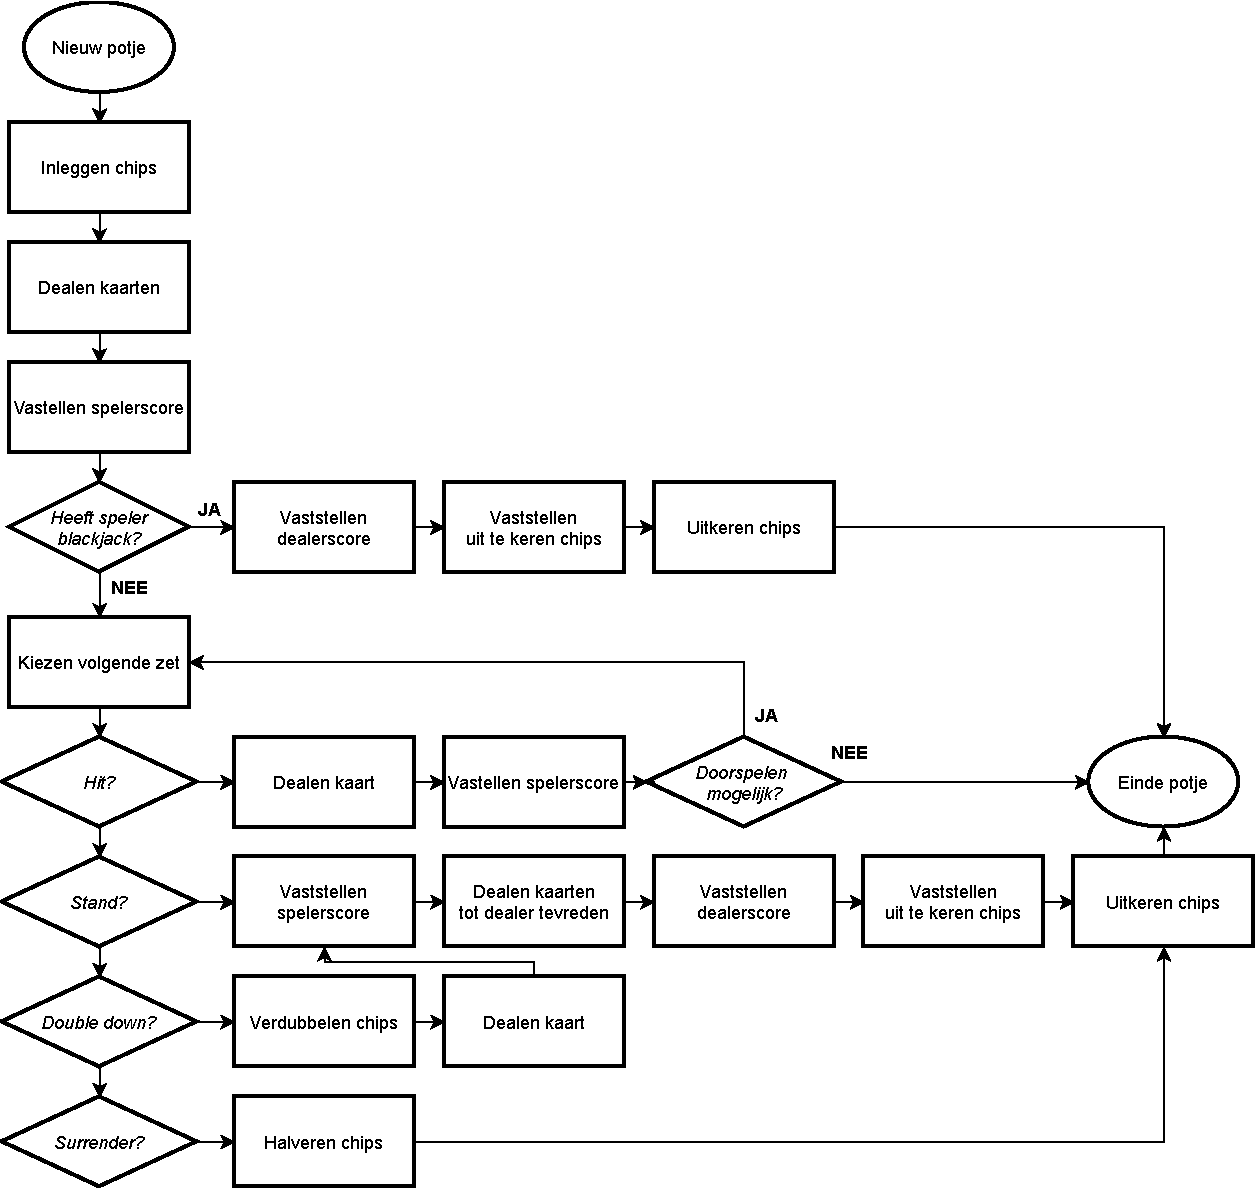
\includegraphics[width=\linewidth]{conceptual-flow-blackjack}
%     \caption{Conceptuele flowchart voor blackjack. 
%     Binnen een web-applicatie zal het er anders uitzien in verband met technische keuzes, efficiëntie en onderhoudbaarheid.}
%     \label{fig:conceptual-flow-blackjack}
% \end{figure}

\subsection{Kaart- en handscore}
Per kaart wordt de score bepaald op basis van de rang (\textit{rank}) van de kaart:

\begin{itemize}
    \item \textbf{Getallen (2 - 10)}: de waarde die erop staat
    \item \textbf{Plaatjes (Jack, Queen, King)}: de waarde 10
    \item \textbf{Aas (Ace): 1 of 11}
\end{itemize}

De handscore wordt bepaald door deze scores bij elkaar op te tellen, 
zie Tabel \ref{table:handscores}.

\begin{table}[H]
    \centering
    \begin{tabularx}{0.4\textwidth}{|l|X|}
        \hline
        \textbf{Kaarten} & \textbf{Handscore} \\ \hline
        $\heartsuit 2, \clubsuit 3$ & 5 \\ \hline
        $\clubsuit 10, \diamondsuit 5, \heartsuit 3, \spadesuit2$ & 20 \\ \hline
        $\heartsuit 10, \clubsuit K$  & 20                 \\ \hline
        $\spadesuit A, \diamondsuit 4$ & 15 (of: 5)         \\ \hline
        $\clubsuit A, \diamondsuit K$ & 21 (of: 11)         \\ \hline
        $\clubsuit A, \heartsuit A$ & 12                 \\ \hline
    \end{tabularx}
    \caption{Voorbeelden van handscores.}
    \label{table:handscores}
    \centering
\end{table}

Merk op dat de aas ertoe leidt dat de speler kan kiezen om 
met de hogere aas-score uit te komen of te hopen op betere kaarten 
met de lagere aas-score. Als de hogere aas-score boven de 21 uitkomt,
hoeven we alleen nog maar te kijken naar de lagere aas-score.

\newpage

\subsection{Speltoestanden}
Er zijn een aantal toestanden waar het spel zich in kan bevinden:
\begin{itemize}
    \item \textit{Waiting}: het spel is aangemaakt, maar nog niet gestart (optioneel)
    \item \textit{Playing}: het spel is gestart en moves kunnen worden geselecteerd
    \item \textit{Bust}: speler heeft een handscore >21 en kan niet meer verder spelen
    \item \textit{Lost}: speler heeft een lagere eindscore dan de dealer
    \item \textit{Surrendered}: speler heeft het opgegeven
    \item \textit{Push}: speler heeft dezelfde handscore als de dealer of beiden hebben een handscore van 21 in de eerste beurt
    \item \textit{Blackjack}: speler heeft een handscore van 21 in de eerste beurt en de dealer niet
    \item \textit{Won}: speler heeft een hogere handscore dan de dealer of de dealer heeft >21
\end{itemize}

\subsection{Uitbetaling}
Het uitbetalen van chips is gebaseerd op de eindtoestand (rond af naar hele chips).
Het spel eindigt alleen bij de volgende speltoestanden:

\begin{itemize}
    \item \textit{Bust}: speler krijgt niets terug
    \item \textit{Lost}: speler krijgt niets terug
    \item \textit{Surrendered}: speler krijgt $0.5\times$ zijn inleg terug
    \item \textit{Push}: speler krijgt $1\times$ zijn inleg terug
    \item \textit{Blackjack}: speler krijgt $1.5\times$ zijn inleg terug
    \item \textit{Won}: speler krijgt $2\times$ zijn inleg terug
\end{itemize}

\newpage

\section{Beoordeling}
Het gaat er bij dit vak om dat je een werkende en structureel goede back-end kan bouwen.
De snelste of kortste oplossing is voor deze cursus (en in de praktijk) niet altijd de beste oplossing!

\subsection{Assessment}
We willen ook dat je je project kunt toelichten 
aan de hand van de voor de leerdoelen relevante behandelde stof.
Dit wordt getoetst aan de hand van een project met bijbehorend interview.

Het is verstandig om je project kort te presenteren met behulp van slides.
Sta daarbij alvast stil bij de theoretische onderbouwing.

\subsubsection{Voorbeeldvragen}
Vragen die je kunt verwachten zijn gebaseerd op de leerdoelen van de cursus.
Je kan denken aan de volgende soort vragen:
\begin{itemize}
    \item Op welke manier heb je \textit{separation of concerns, loose coupling en high cohesion} bereikt?
    \item Wat houdt \textit{<object model element, design principle, design pattern>} in?
    \item Op welke manier heb je \textit{<design principle>} toegepast?
    \item Waarom zou je \textit{<object model element, design principle, design pattern, dependency injection>} gebruiken?
    \item Hoe heb je \textit{<design pattern>} in dit project uitgevoerd?
    \item Welk \textit{<design pattern>} zou je op \textit{<projectonderdeel>} kunnen toepassen?
    \item Op welke manier voldoe je aan \textit{<REST principe>}?
    \item Wat is de verantwoordelijkheid van \textit{<laag X>}?
\end{itemize}

\section{Rubric}
Zie Canvas voor de rubric van het project. Heb je alle punten gehaald, dan haal je een 10.
Mocht je wat minder scoren op bepaalde onderdelen, dan wil dat niet zeggen dat je een onvoldoende hebt!
Hier kan je natuurlijk rekening mee houden wanneer je met een planning bezig gaat.
\chapter{Opdracht 1: Projectopzet en analyse}

\section{Stap 1: Zet het project op}
Gebruik voor het project \textit{Java}, versie 11 of hoger.

Verder gebruiken we \textit{Maven}, een tool waarmee je Java-projecten kan opzetten
en gemakkelijk third-party dependencies, zoals frameworks en libraries, kunt 
gebruiken in je project. Zie hiervoor de pom.xml. Maven hoef je niet per se te 
installeren. We kunnen hiervoor onze Integrated Development Environment (IDE) gebruiken.
Ook is er een wrapper (mvnw) opgenomen in het project mocht je de commandline willen gebruiken (aanrader!). 

\subsection{Clone het project}
Clone het GitHub-project via de link die op Canvas wordt aangeboden.
We gebruik hiervoor private repositories binnen GitHub Education.
Zorg dat je een clone krijgt binnen GitHub om je werk in te leveren 
en op je machine om te werken. Open de root-directory van het project
via IntelliJ.

\subsection{Neem de opdrachtbeschrijving door}
Neem de opdrachtbeschrijving en de opdracht op Canvas door. 
Kan je (voor jezelf) antwoord geven op de volgende vragen?

\begin{enumerate}
    \item Wat moeten we precies maken?
    \item Waarom is er gekozen voor een web-applicatie?
    \item Hoe werkt blackjack ongeveer?
    \item Wat ga je ongeveer leren met deze cursus?
    \item Waar word je op beoordeeld?
    \item Waar krijg je de meeste punten voor?
    \item Wat moet je doen voor een voldoende?
\end{enumerate}

In het verleden is gebleken dat veel studenten erg laat beginnen 
en daarmee in de knoop komen met andere cursussen. Probeer dat te 
voorkomen door regelmatig je werk in te leveren, zodat je continu feedback 
kunt krijgen. Het is dus handig om voor jezelf een planning te maken.
De opdracht is om die reden opgedeeld in 6 stappen die ongeveer gelijk lopen 
met de inhoudelijke invulling van de werkcolleges.
Maak je je op enig punt tijdens de cursus zorgen over de planning,
geef het aan!

\subsection{Extra informatie: de projectstructuur}
Studenten hebben aangegeven meer informatie te willen ontvangen over hoe het 
systeem is opgezet. Daar is dit onderdeel voor bedoeld. Het is niet 
erg als je nog niet alles helemaal begrijpt of dat je niet overtuigd 
bent van deze opzet. Het gaat erom dat je in hoofdlijnen doorhebt 
waar wat te vinden is. Tijdens deze cursus gaan we er dieper op in.

Laten we eens kijken naar hoe het project is opgezet.
Onder src/main/java zien we onze packagestructuur.
Met behulp van packages kunnen we ons systeem op een logische manier 
ordenen. Dit is een belangrijke stap in het bereiken van 
\textit{separation of concerns, high cohesion en loose coupling}!

Structurele kwaliteit ziet immers op de onderhoudbaarheid
van een softwareproject. Een softwareproject heeft in algemene zin 
een goede structuur als deze is opgedeeld in kleine,
opzichzelf staande modules die intern veel samenhang 
en met elkaar beperkt koppeling vertonen.

\subsubsection{Packagestructuur in Java}
In Java kunnen we modules groeperen door gebruik te maken van 
\emph{packages} (in C\# en andere talen met \emph{namespaces}).
De naam van een Java-package lijkt op een soort omgekeerd webadres
en komt overeen met de onderliggende mappenstructuur.
Het is gebruikelijk om in Java-packages eerst te beginnen met de organisatienaam,
bijvoorbeeld \texttt{nl.hu.bep2}, en vervolgens de projectnaam \texttt{casino}.
Dan kunnen we het project opdelen in componenten, zoals in het casino-project: 
\begin{itemize}
\item \texttt{nl.hu.bep2.casino.chips}
\item \texttt{nl.hu.bep2.casino.blackjack}
\item \texttt{nl.hu.bep2.casino.security} (later)
\end{itemize}

Binnen elk component kan met packages 
onderscheid gemaakt worden naar het soort logica volgens een gelaagde aanpak. 
Dat leidt bij het casino-project tot de volgende 
mappen- en packagestructuur onder \texttt{src/main/java}:

\dirtree{%
    .1 nl.hu.bep2.casino.
        .2 chips.
            .3 application.
            .3 domain.
                .4 exception.
        .2 blackjack.
            .3 (...).
}

Het project is dus eerst opgedeeld in verschillende componenten en vervolgens in 
lagen. Voor nu is de splitsing in lagen gebaseerd op een 'application'-laag waarin 
we expliciet de verschillende usecases een plekje geven, en een 'domein'-laag waar 
we een domeinmodel realiseren (de ingrediënten van de usecases, zeg maar).

\subsection{Voorbeeld: Use cases van het chips-component}
Het chips-component biedt al een aantal use cases aan binnen ons systeem.
Deze zijn opgesomd in de ChipsService en laten zich gemakkelijk in een 
use case diagram vatten, zie: Figuur~\ref{fig:chips-use-cases}.
Kijk in de code of je dit kunt herkennen!

\begin{figure}[H]
    \centering
    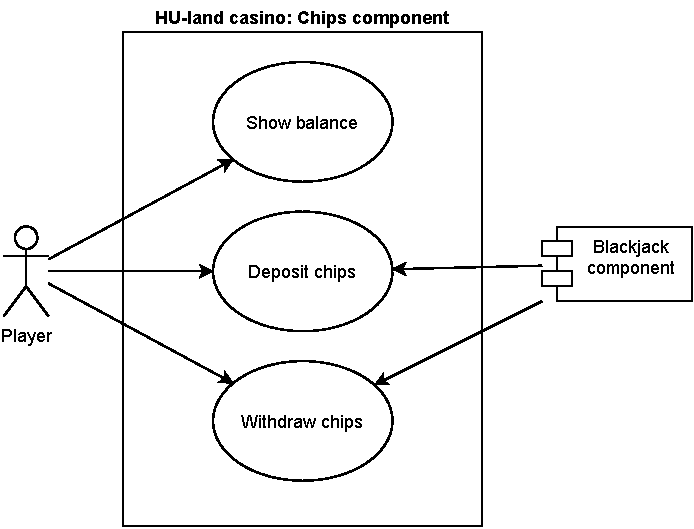
\includegraphics[height=0.4\linewidth]{chips-use-cases}
    \caption{De use cases van het chips-component}
    \label{fig:chips-use-cases}
\end{figure}

Zoals je ziet, willen we onze blackjack-component straks 
ook gebruik laten maken van de de chips-component!

\section{Stap 1: Analyseer de use cases van blackjack}
We hebben de opdracht doorgenomen en weten wat de opdrachtgever van ons verwacht.

We moeten ons voorstellen hoe blackjack precies werkt in de echte wereld.
Daarvan willen we een model maken in diagrammen en code, maar ook in ons hoofd!

Laten we een use case diagram maken, zodat de acties die door het systeem
aangeboden moeten worden voldoende duidelijk zijn. Hiervoor kan je het use case 
diagram van Figuur~\ref{fig:chips-use-cases} als inspiratie nemen.

\begin{figure}[H]
    \centering
    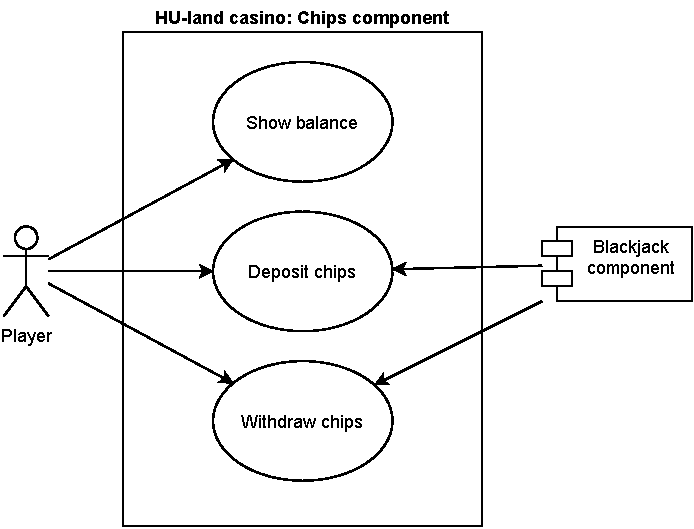
\includegraphics[height=0.4\linewidth]{chips-use-cases}
    \caption{De use cases van het chips-component}
    \label{fig:chips-use-cases}
\end{figure}

Neem de opdrachtbeschrijving door en denk na over de volgende zaken:
\begin{enumerate}
    \item Welke actors zijn er? Geautomatiseerde actors hoef je niet op te nemen.
    \item Wat wordt er binnen het component allemaal afgehandeld? Dit zijn geen use cases!
    \item Welke use cases moeten er naar buiten toe aangeboden worden om blackjack te kunnen spelen?
\end{enumerate}

Gebruik een tool als \textit{diagrams.net}, \textit{software ideas modeler} of \textit{visual paradigm},
sla het ontwerp op en exporteer het als \textit{.png} of \textit{.jpg}. 
Neem dit op in je projectdirectory (bijvoorbeeld onder een mapje \textit{diagrams}),
zodat je docent er naar kan kijken en er feedback op kan geven.

Commit je wijzigingen met een duidelijke naam, 
bijvoorbeeld: "Add use case diagram for blackjack". 
Push de wijzigingen naar je remote GitHub repository.

\section{Het objectmodel}
Wanneer je werkt met objecten, is het goed om het objectmodel van Booch in 
het achterhoofd te houden.\footnote{
    In de praktijk wordt ook wel eens verwezen naar de \textit{4 Pillars of Object Orientation}: 
    abstraction, encapsulation, polymorphism en inheritance. 
    Deze zijn in het objectmodel van Booch inbegrepen.
}

Het objectmodel van Booch onderscheidt vier belangrijke elementen 
die een rol spelen bij het object-georiënteerd modelleren:
\begin{enumerate}
    \item Abstraction
    \item Encapsulation 
    \item Modularity 
    \item Hierarchy
\end{enumerate}

Deze onderdelen noemen Booch et al. belangrijk omdat je 
zonder deze elementen geen object-georiënteerde taal (OO-taal) kan hebben.
Daarnaast beschrijven zij drie minder belangrijke elementen die je 
bij veel OO-talen tegen kunt komen: typing, persistence en concurrency.

Dit betekent natuurlijk niet dat je deze zaken buiten OO-talen niet tegen zal komen! 
Het objectmodel van Booch onderscheid een aantal zaken
die ons helpen goed gestructureerde object-georiënteerde software te ontwerpen.

Dit komt tijdens de colleges aan bod, maar kunnen we als volgt samenvatten:
\begin{enumerate}
    \item \textbf{Abstraction}: klassen en objecten zijn onze kernabstracties waarin we 
    toestand (fields) en gedrag (methods) samenbrengen die bij elkaar horen. Dit verhoogt \textit{cohesion}.
    We kunnen met deze abstracties communiceren via de publieke methoden. 
    De interne werking hoeven we dan niet te weten (\textit{implementation hiding}).
    \item \textbf{Encapsulation}: hoe een abstractie zijn toestand bijhoudt en zijn 
    gedrag uitvoert wordt afgeschermd van de buitenwereld. Om \textit{information hiding} te bereiken wordt 
    gebruik gemaakt van access modifiers (bijvoorbeeld: \textit{private}). 
    Dit beperkt \textit{coupling}. Wees spaarzaam met getters en setters (\textit{Tell, don't Ask}) 
    en wees niet afhankelijk van de onderdelen binnen een klasse \textit(\textit{Law of Demeter}).
    \item \textbf{Modularity}: klassen zijn modules waarin we toestand en gedrag samenbrengen. Daarnaast kennen 
    we interfaces om bepaald gedrag af te dwingen en enums om mogelijke waarden op te sommen. 
    Packages kunnen we gebruiken om klassen en andere modules te ordenen.
    \item \textbf{Hierarchy}: we kunnen packages onderbrengen in een logische, overzichtelijke ordening. Dat is onderdeel 
    van een softwarearchitectuur. Ook klassen en objecten kunnen in een hiërarchie tot elkaar staan. Er zijn namelijk 
    verschillende afhankelijkheden die tussen klassen kan gelden: \textit{dependency}, \textit{association}, \textit{aggregation},
    \textit{composition}, \textit{inheritance} en \textit{realisation}. Wat betreft inheritance en realisation zorgen 
    \textit{subtyping}, \textit{polymorphism} en \textit{dynamic binding} ervoor dat we een flexibele, uitwisselbare 
    invulling kunnen hebben van bepaalde abstracties. Eén abstractie kan namelijk verschillende vormen aannemen tijdens runtime:
    een subtype kan een implementatie of overschrijving verzorgen van het supertype.
\end{enumerate}

\section{Stap 2: Ontwerp een globaal domeinmodel}
Zodra je hebt nagedacht over de use cases en hier een model van hebt gemaakt,
kunnen we een overzicht maken van de concepten die we nodig hebben in ons blackjack-component.

Hiervoor kunnen we een versimpeld domeinmodel maken. 
Methods, attributes, rolnamen en multipliciteiten mag je achterwege laten.
Wees niet bang om veel concepten te modelleren!

Loop nogmaals door de opdrachtbeschrijving en verwerk de volgende zaken in je 
domeinmodel:
\begin{enumerate}
    \item Welke concepten leven er in de wereld van blackjack? 
    \item Wat zijn goede kandidaten voor klassen en enums?
    \item Wat zijn de relaties tussen deze concepten? Geef dit aan met de juiste pijlen.
    \item Welk concept kunnen we als centraal aanspreekpunt aanmerken waar we andere concepten aan kunnen hangen?
\end{enumerate}

Probeer hier niet teveel tijd aan te besteden.
Dit is een eerste opzet om het domein te structureren.
Tijdens het programmeren leren we meer over het domein, de functionaliteit en de structuur
en gaan we dit nader invullen en aanpassen!

Gebruik een tool als \textit{diagrams.net}, \textit{software ideas modeler} of \textit{visual paradigm},
sla het ontwerp op en exporteer het als \textit{.png} of \textit{.jpg}. 
Neem dit op in je projectdirectory (bijvoorbeeld onder een mapje \textit{diagrams}),
zodat je docent er naar kan kijken en er feedback op kan geven.

Commit je wijzigingen met een duidelijke naam, 
bijvoorbeeld: "Design initial domain model for blackjack". 
Push de wijzigingen naar je remote GitHub repository.

De docent geeft algemene of specifieke feedback
op basis waarvan je je domeinmodel kunt verbeteren.
Wat we alvast kunnen weggeven is dat je een spelpotje 
als centrale domeinklasse kan nemen.

\chapter{Opdracht 2: Domeinmodel implementeren}

\section{Stap 3: Realiseer eerste domeinconcepten}
Het kan handig zijn om met deze stap te beginnen als je al wat feedback hebt 
gehad op je domeinmodel, maar je kan natuurlijk alvast beginnen en het na 
de feedback verbeteren.

We gaan de basis van ons domein leggen door alvast wat klassen aan te maken.
De methodes kunnen we nu al toevoegen, maar dit kunnen we ook later doen. 
Alvast een tip: probeer nog geen getters of setters te maken. 
Setters heb je meestal niet nodig en getters maken we pas aan wanneer
we de data daadwerkelijk uit een object moeten halen. Dit is eigenlijk alleen 
het geval wanneer je een soort vertaalslag moet uitvoeren, bijvoorbeeld tussen 
lagen of tussen ons systeem en de buitenwereld.

Laten we eerst weer de IDE induiken en beginnen met packages aan te maken!
Deze packages hebben een betekenisvolle rol in onze architectuur: 
we willen separation of concerns, high cohesion en loose coupling.

\subsection{Maak packages}
In IntelliJ kan je packages aanmaken door met de rechtermuisknop op de package
in het projectoverzicht (links) te klikken waar je iets nieuws wil toevoegen
en dan naar \texttt{New > Package} te gaan 
(je kan ook `package' typen of de pijltjestoetsen gebruiken). 
Als alternatief kan je ook de parent-package selecteren en dan 
het generate-scherm openen met \texttt{ALT + INSERT} (MacOS: \texttt{COMMAND + N}). 

Maak een nieuwe package aan: \texttt{nl.hu.bep2.casino.blackjack}.
Dit is de package voor ons component, ons deelgebied, dat over blackjack zal gaan.
We zijn bezig met het modelleren van het domein. Laten we daarvoor een laag aanmaken.
Ook daarvoor maken we een package: \texttt{nl.hu.bep2.casino.blackjack.domain}.

In deze package zouden we nog subpackages kunnen aanmaken, bijvoorbeeld om zaken te groeperen.
Denk bijvoorbeeld aan concepten die herbruikbaar zijn voor allerlei soorten kaartspellen 
in plaats van alleen voor blackjack. Dan zouden we een package kunnen aanmaken: 
\\ \texttt{nl.hu.bep2.casino.blackjack.domain.cards}. Dit kunnen we ook doen zodra we 
wat verder zijn en bekend is welke concepten er in ons domein leven.

Let op: packagenamen schrijven we in Java altijd met kleine letters,
zonder leestekens!

\subsection{Voeg klassen en enums toe}
Laten we beginnen met één centrale klasse dat ons aanspreekpunt wordt
voor domeinacties. Die klasse wordt ook het uitgangspunt wanneer we het gaan opslaan.

Maak deze centrale klasse aan. Selecteer in het projectoverzicht de 
package waaraan je een klasse wil toevoegen en klik rechtermuisknop, \texttt{New > Class}. 
Ook hier kan je hotkeys gebruiken: \texttt{ALT + INSERT} (MacOS: \texttt{COMMAND + N}).
Laten we het een Engelse naam geven dat spelpotje betekent (bijvoorbeeld: \texttt{Game} of \texttt{Table}).

Let op: klasse-, interface, en enum-namen schrijven we in Java altijd met in Pascal-case 
(\textit{StudlyCaps}), zonder leestekens!

Wat moet een spelpotje allemaal gaan bijhouden? Probeer dit op te nemen in de fields.
We willen bijvoorbeeld het huidige pakje speelkaarten bijhouden voor dit spelpotje.
Zorg dan dat je klasse er als volgt uit ziet. Vraag je af: waarom declareren we dit veld als \textit{private}?

\begin{minted}{java}
    package nl.hu.bep2.casino.blackjack.domain;

    public class Game {
        private Deck deck;
    }
\end{minted}

Als het goed is, is \texttt{Deck} in IntelliJ roodgekleurd 
of voorzien van een waarschuwing. Leer dit soort signalen te herkennen!
Om de \texttt{Deck} aan te maken, kan je met je cursor (of caret) op de het
type gaan staan (\texttt{Deck}) en de klasse laten genereren door de hotkeys
\texttt{ALT + ENTER} (MacOS: \texttt{OPTION + ENTER}) te gebruiken 
(show intention actions). Selecteer `create class' en geef de package aan 
waar je de klasse in wil aanmaken. Druk op \texttt{ENTER}.

\subsection{Vul de rest van de objectboom in}
Voeg vervolgens op deze zelfde manier alle andere velden (en de bijbehorende klassen) toe 
die deze centrale \texttt{Game}-klasse nodig heeft.
Voeg ook de velden toe van de velden van deze klasse en herhaal dit proces totdat
je je objectboom klaar hebt.

Je zou \texttt{Deck} kunnen voorzien van een verzameling van kaarten 
en een kaart weer van een rang en een kleur. Denk na over hoe je rang en kleur en 
handigst in Java kunt programmeren op een leesbare en herbruikbare manier.
Er is een manier die ervoor zorgt dat je nooit een kaart kan maken met een niet-bestaande 
rang of kleur. Er zijn maar 52 mogelijkheden: 4 kleuren en 13 rangen.

Je mag ook al methodes aanmaken, maar het gaat ons nu vooral om een eerste structuur.
We weten pas hoe de methodes precies werken zodra we onze use cases implementeren 
in een applicatie service (zie volgende opdracht).

Commit je wijzigingen met een duidelijke naam, 
bijvoorbeeld: "Structure initial domain concepts". 
Push de wijzigingen naar je remote GitHub repository.

\subsection{Maak constructors aan}
Maak voor elke klasse in ons domein een constructor aan.
Een constructor is een speciaal soort (statische) methode die wordt aangeroepen
om een objectinstantie te maken. Daar kunnen we ook instanties aan meegeven om 
de velden te vullen.

Ook constructors kan je genereren. Zet je cursor op een veld en klik 
rechtermuisknop `Show Context Actions' of gebruik de hotkey \texttt{ALT + ENTER} 
(MacOS: \texttt{OPTION + ENTER}) terwijl je caret op een veld staat. 
Je kan ook willekeurig op een plek in je klasse je caret neerzetten en iets genereren 
met \texttt{ALT + INSERT} (MacOS: \texttt{OPTION + N}).

Nu opent er een scherm om een constructor te genereren op basis van de velden. Je kan 
gemakkelijk alle velden selecteren door \texttt{SHIFT} ingedrukt te houden en 
pijltje naarbeneden te doen totdat je alle velden geselecteerd hebt. Vervolgens kan je 
op \texttt{ENTER} drukken om je keuze te bevestigen. Dan krijg je nog wat opties om de 
constructor aan te passen, maar meestal hoeft dat niet. Druk nogmaals op \texttt{ENTER}.

\begin{minted}{java}
    package nl.hu.bep2.casino.blackjack.domain.cards;

    public class Deck {
        private List<Card> cards;

        public Deck(List<Card> cards) {
            this.cards = cards;
        }
    }
\end{minted}

Je kan ook waarden initialiseren in de velden zelf. Dan hoef je ze niet mee te geven 
in de constructor, maar heeft een veld een bepaalde startwaarde wanneer een object 
geïnitialiseerd wordt. Denk bijvoorbeeld aan een lijst van kaarten, zoals in een Deck.
Als je met een lege Deck wil beginnen kan je het volgende doen:

\begin{minted}{java}
    package nl.hu.bep2.casino.blackjack.domain.cards;

    public class Deck {
        private List<Card> cards = new ArrayList<>();
    }
\end{minted}

Wil je een nieuw veld toevoegen aan een bestaande constructor? Declareer dan eerst het veld
en ga vervolgens met je caret op dit (grijze) veld staan. 
Doe wederom \texttt{ALT + ENTER} (MacOS: \texttt{OPTION + ENTER})
en kies `Add constructor parameter'.

Commit je wijzigingen met een duidelijke naam, 
bijvoorbeeld: ``Add constructors to domain concepts''. 
Push de wijzigingen naar je remote GitHub repository.

\subsection{Tip: een named constructor toevoegen aan Deck}
Beginnen met een lege Deck en van buitenaf allerlei kaarten toevoegen 
(bijvoorbeeld in de constructor of een \texttt{add(Card card)} methode)
is misschien niet de meest praktische oplossing.

Waarschijnlijk willen we elke keer als we een nieuwe Deck maken
deze vullen met kaarten. Daarvoor kunnen we een zogenaamde \textit{named constructor}
maken: een static method op \texttt{Deck} die een \texttt{Deck} teruggeeft 
na alle kaarten toegevoegd te hebben. Om een volle deck terug te geven, zouden 
we een functie met de volgende vorm kunnen aanmaken:

\begin{minted}{java}
public class Deck {
    private List<Card> cards = new ArrayList<>();

    public static Deck full() {
        Deck deck = new Deck();

        // TODO: Creation of all cards and adding them to the deck

        return deck;
    }
}
\end{minted}

Binnen de \texttt{full}-methode kunnen we kaarten toevoegen aan de 
deck-instantie door \texttt{deck.cards.add(card)} te doen. De \texttt{card}
moet je dan wel zelf aanmaken.

Hoe je precies de kaarten moet aanmaken en toevoegen aan de Deck,
laten we nog even aan jou. Afhankelijk van hoe je de kaarten gemodelleerd hebt 
in je spel, kan je dit oplossen zonder alle 52 kaarten met de hand te benoemen!

\subsection{Voeg al wat methods toe}
Het is goed om alvast wat gedrag toevoegen aan de objecten!
Maar wees niet bang om ze later aan te passen of te verwijderen.
Overbodige code is dode code.

Naast welke objecten precies welke verantwoordelijkheid hebben 
kunnen we ook nadenken over het gedrag dat zij aanbieden; 
het domein is meer dan slechts met getters en setters data heen en weer te schuiven. 
Een algemene tip is om te denken in gedrag in plaats van data. 
Setters heb je eigenlijk bijna niet nodig, getters alleen wanneer je ze aanroept. 

Probeer het object op zichzelf te beschouwen: welke vragen (queries) zou je eraan willen stellen? 
Welke acties (commands) zou je het willen laten uitvoeren? 
Waar bestaat het object uit en moet het object met andere objecten samenwerken? 
Andere objecten waarmee samengewerkt wordt, afhankelijkheden, 
kunnen we het beste in de constructor meegeven of als parameter van de methode die wordt aangeroepen. 
Het doel is om te komen tot een goed georganiseerde objectstructuur met één duidelijk aanspreekpunt: 
een game object dat later kan worden opgeslagen. 
Dit game object heeft kennis van allerlei onderliggende domeinconcepten 
die elk hun eigen specifieke verantwoordelijkheid hebben. 
Wees niet bang om veel objecten aan te maken met kleine methodes per specifieke actie! 
Ook hier komen de eigenschappen van het objectmodel om de hoek kijken.

Je kan je klassen testen door gebruik te maken van JUnit of het even 
in een Main-functie uit te proberen. We gaan het later handmatig testen met 
Postman. In een latere cursus gaan we dieper op het correct testen van object-georiënteerde projecten in.

\subsection{Tip: Gebruik je IDE!}
Wil je een klasse of package verplaatsen, versleep deze dan in het projectoverzicht.
Alle imports en verwijzingen worden automatisch geupdate. Wil je hiervoor een hotkey gebruiken,
dan is dat \texttt{F6} (MacOS: \texttt{F6}) terwijl je het betreffende item hebt geselecteerd 
in het projectoverzicht of open hebt staan in de editor. Je kan ook gebruik maken van 
het refactor-menu door rechtermuisknop op een klasse of package te doen.

Wil je een klasse of package hernoemen, dan kan je rechtermuisknop 
\texttt{Refactor > Rename} doen of de hotkeys \texttt{SHIFT + F6} (MacOS: SHIFT + F6).
Dezelfde hotkey kan je gebruiken om velden, variabelen en methoden te hernoemen.

Gebruik voor dit soort zaken altijd je IDE! Dit bespaart je een hoop tijd omdat je IDE 
het op allerlei plekken tegelijkertijd voor je aanpast. Op het hele project kan slim gebruik 
van je IDE je uren besparen! 

Er zijn nog meer van dit soort hotkeys. 
Voor een overzicht, zie: \href{https://www.jetbrains.com/help/idea/reference-keymap-win-default.html}{Windows hotkeys} 
of \href{https://www.jetbrains.com/help/idea/reference-keymap-mac-default.html}{MacOS hotkeys}.

Heb je geen zin om steeds de handleiding of Google te gebruiken? Dan kan je altijd de hotkey 
\texttt{CTRL + SHIFT + A} gebruiken om een trefwoord te typen van wat je wil doen.
Vaak geeft IntelliJ een goede suggestie. 

Wil je geïnformeerd worden wanneer je iets doet waar je een hotkey voor had kunnen gebruiken?
Dan kan je de IntelliJ-plugin Keypromotor X installeren, zie 
\href{https://www.jetbrains.com/help/idea/mastering-keyboard-shortcuts.html#learn-shortcuts}{IntelliJ's uitleg}.

\chapter{Opdracht 3: Application service}
We hebben het project aan de praat, de eisen geanalyseerd, 
de use cases gemodelleerd en de eerste domeinconcepten gerealiseerd. 
Het doet allemaal alleen nog niet zoveel!

\section{Spring Boot}
Spring Boot is een veelgebruikte standaardconfiguratie van het Spring framework. 
Vanaf gaan we ons mooie java-domein-model aanspreken met een echte Webservice.

In deze fase gebruiken we al wel de HTTP-functionaliteit van Spring (@RestControllers), maar
de database is er nog niet. Daarvoor gebruiken we een In-memory nep-implementatie. Voorlopig 
zal dus alle data ge-reset zijn elke keer dat je de applicatie opnieuw opstart (maar geen zorgen
dat pakken we later weer op!).

\subsection{Project Structuur}

Ondertussen is de mappen- en packagestructuur onder \texttt{src/main/java} een stuk uitgebreider geworden:

\dirtree{%
    .1 nl.hu.bep2.casino.
        .2 chips.
            .3 presentation.
                .4 controller.
                .4 dto.
            .3 application.
            .3 domain.
                .4 exception.
            .3 data.
        .2 security.
        .2 blackjack.
            .3 (...).
}

Het project is dus eerst opgedeeld in verschillende componenten en vervolgens in 
lagen. In lagen kunnen we zaken weer groeperen in deelsystemen. Deze componenten 
en lagen kunnen we weergeven als packages, zie Figuur~\ref{fig:uml-casino-physical-layers}.

\begin{figure}[H]
    \centering
    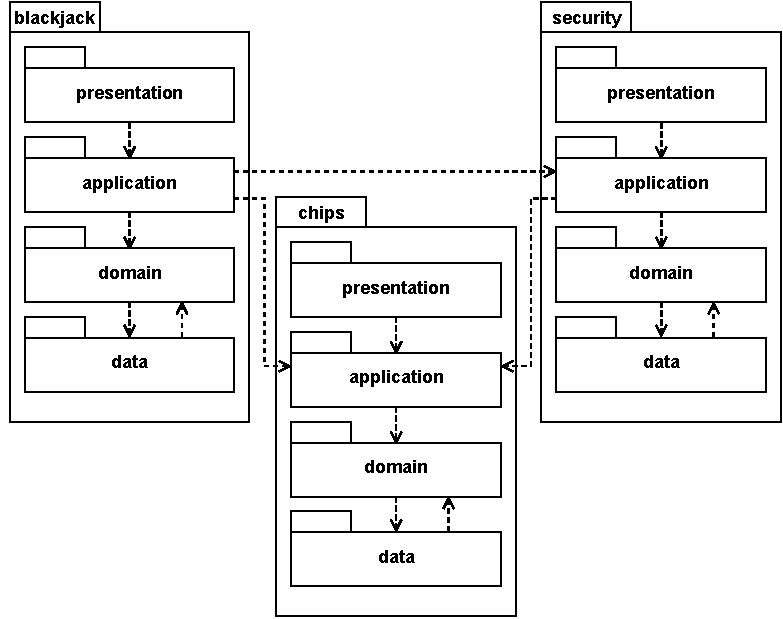
\includegraphics[width=.6\linewidth]{uml-casino-physical-layers}
    \caption{Components en layers kunnen met packages worden aangewezen binnen het casinoproject.}
    \label{fig:uml-casino-physical-layers}
\end{figure}

\subsubsection{Componenten}
Een component is een opzichzelfstaand onderdeel van een softwaresysteem
dat ziet op een bepaald deelgebied aan functionaliteit, bijvoorbeeld op een 
bepaald subdomein.

Het component bevat een aantal domeinobjecten. 
De communicatie wordt aangeboden via een service (ook: \textit{facade}). 
Deze service kan worden aangesproken door andere
services, maar ook door bijvoorbeeld een controller of een commando uit een commandline interface. 
De controller is bedoeld om HTTP-communicatie om te zetten naar Java code en vice versa. 
Andersom praat het component alleen met de buitenwereld, zoals een database, via een \textit{gateway}.

In ons project maken we gebruik van Spring om controllers te schrijven.
Deze controllers kunnen dan door Spring worden aangeroepen 
wanneer een bepaald web request moet worden afgehandeld.
Aan de andere kant maken we later ook gebruik van Spring om te voorzien in 
de data-opslag aan de hand van repositories.

\subsubsection{Lagen}
Een applicatie, of een deel ervan, is vaak opgedeeld in lagen die 
elk verantwoordelijk zijn voor een ander soort logica binnen het systeem.
Het afhandelen van gebruikersinteractie 
is bijvoorbeeld iets heel anders dan het uitdelen van kaarten in een
kaartspel of het opslaan van een speelronde.
Een gelaagde structuur helpt niet alleen met het terugvinden van
bepaalde klassen op basis van het soort logica dat het betreft. Bij een 
losgekoppeld ontwerp kunnen lagen of onderdelen ervan gemakkelijk uitgewisseld worden.

Gelaagde architecturen komen in verschillende soorten en maten. Sommige applicaties 
zijn eerst opgesplitst in componenten en vervolgens ingedeeld in lagen. Andere zijn 
eerst opgesplitst in lagen, waarin vervolgens losse componenten zijn te bespeuren.
Het aantal lagen kan variëren tussen de twee en vijf lagen. Dit hangt af 
van de verschillende soorten logica en de specifieke architecturele eisen
van de onderdelen binnen een project.

Deze packages corresponderen met de volgende soorten logica:
\begin{itemize}
    \item \emph{Presentation}: Presentatielogica. In het geval van een back-end API tref
    je hier alles aan dat hoort bij de technische vertaling van web requests naar Java-code. 
    Controllers (web request handlers) worden aangeroepen door het Spring framework 
    zodra een HTTP-request binnenkomt met een gedefinieerde route (HTTP-method + URL).
    \item \emph{Application}: Taakspecifieke logica. Hierin zitten applicatieservices (\emph{facades}) 
    die use cases omzetten naar domeinacties met behulp van infrastructuurabstracties. Een applicatieservice
    ziet vaak op één centraal domeinobject dat is opgebouwd uit of verwijst naar andere domeinobjecten.
    Door een applicatielaag in te richten kan dezelfde logica geboden worden onafhankelijk van de gebruikte 
    technologie in de presentatielaag: command line commando's, GUI's, web controllers of message handlers.
    \item \emph{Domain}: Domeinlogica. Domeinconcepten, business rules en entiteiten vind je vaak in lagen 
    met deze verantwoordelijkheid.
    \item \emph{Data}: Infrastructuurabstractie. Hierin zitten meestal interfaces of abstracte klassen die door
    infrastructuurklassen moeten worden ingevuld (\emph{gateways}).
\end{itemize}

Probeer voor jezelf de volgende vragen te beantwoorden, eventueel door naar de code te kijken.
Welke klasse is verantwoordelijk voor de vertaling van HTTP-verkeer naar Java en andersom?
In welke klassen zal je de use cases van dit component terugzien?
In welke methode wordt het aantal chips verminderd bij een afschrijving?
Hoe denk je dat de opslag geregeld is?
Stel een ander component binnen ons systeem wil Chips opnemen voor een user, welke klasse wordt dan 
eerst aangesproken?

Je mag dit met docenten en medestudenten overleggen, 
maar het antwoord op deze vragen zal naar verloop van tijd duidelijker worden.

\subsubsection*{Kanttekening: Geen écht lagenmodel}
Het casinoproject is opgezet met de verschillende soorten logica in gedachten. 
Als je het lagenmodel echter strikt zou toepassen op Figuur~\ref{fig:uml-casino-physical-layers}, 
zie je een overtreding in de laatste twee lagen van elk component. 
Hier gaan we later in dit collegejaar op in (bij de cursus \textbf{Software Architecture}),
maar misschien wil je hier al wat meer over weten.

De datalaag bestaat weliswaar slechts uit interfaces die door 
Spring geïmplementeerd worden, maar ze zijn afhankelijk van objecten (entiteiten) die
gedefinieerd zijn in het domein. Logisch gezien zou je het project daarom 
eerder beschouwen als een drie-lagen-architectuur! De laatste laag zou dan 
conceptueel zowel domeinlogica als infrastructuurabstracties bevatten. 
Deze laag is dan fysiek (in onze code) opgedeeld in twee Java packages 
om de abstracte, stabiele kern (domein) te scheiden van de meer flexibele 
aansluiting met infrastructuur via interfaces (data). 
Het casino-project kent verder een flexible layered architecture: 
je mag lagen overslaan.
Zo mag je in de presentatielaag een domeinobject teruggeven,
zodat het in een HTTP-response kan worden opgenomen, en exceptions uit het domein 
afhandelen zodat een HTTP-response de juiste statuscode kan hebben.
Dit is in veel gelaagde architecturen niet het geval. In die architecturen 
heeft een laag alleen koppeling met de laag rechtstreeks eronder.
In ons project is dit niet nodig. Het scheelt een hoop extra code en we 
tolereren de extra koppeling.

\begin{figure}[H]
    \centering
    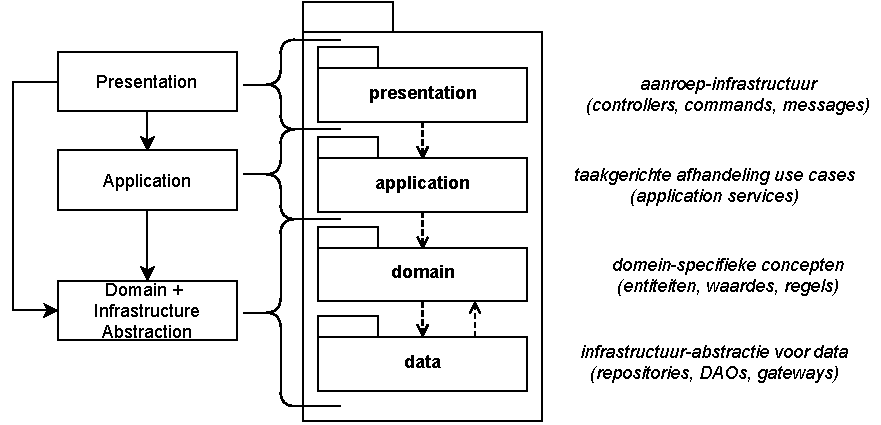
\includegraphics[width=.7\linewidth]{casino-layers}
    \caption{Het logisch en fysiek lagenmodel binnen het componenten van het casinoproject.}
    \label{fig:casino-layers}
\end{figure}

Als je de realisatie toch meer wil afstemmen op de laging, zou je de 
data-objecten en domein-objecten van elkaar splitsen en deze als losse objecten opnemen in de datalaag.
Daarvoor moet je dan daartussen een vertaalslag aanbieden. 
Als je daarnaast wil verbieden dat er lagen worden overgeslagen, 
zou je ook een vertaalslag kunnen toevoegen tussen domeinobjecten en presentatie-objecten.
Als alternatief zou je de infrastructuur-abstractie
(de repositories) kunnen opnemen in het domein en dat \textit{data} package verwijderen.
In ons project passen we deze regels echter niet zo strikt toe:
we accepteren een lichte koppeling op het framework en op ons domein.

\subsubsection{Subsystems}
Een laag kan nog verder worden opgebroken in subsystems (of \textit{deelsystemen}).
Dit zijn algemene packages die zijn bedoeld om een reeks objecten samen te verpakken.

\subsection{Voorbeeld: Structuur binnen het chips-component}
Elk component is in lagen opgedeeld. In het chips-component ziet 
dat eruit zoals in Figuur~\ref{fig:chips-layers}.

\begin{figure}[H]
    \centering
    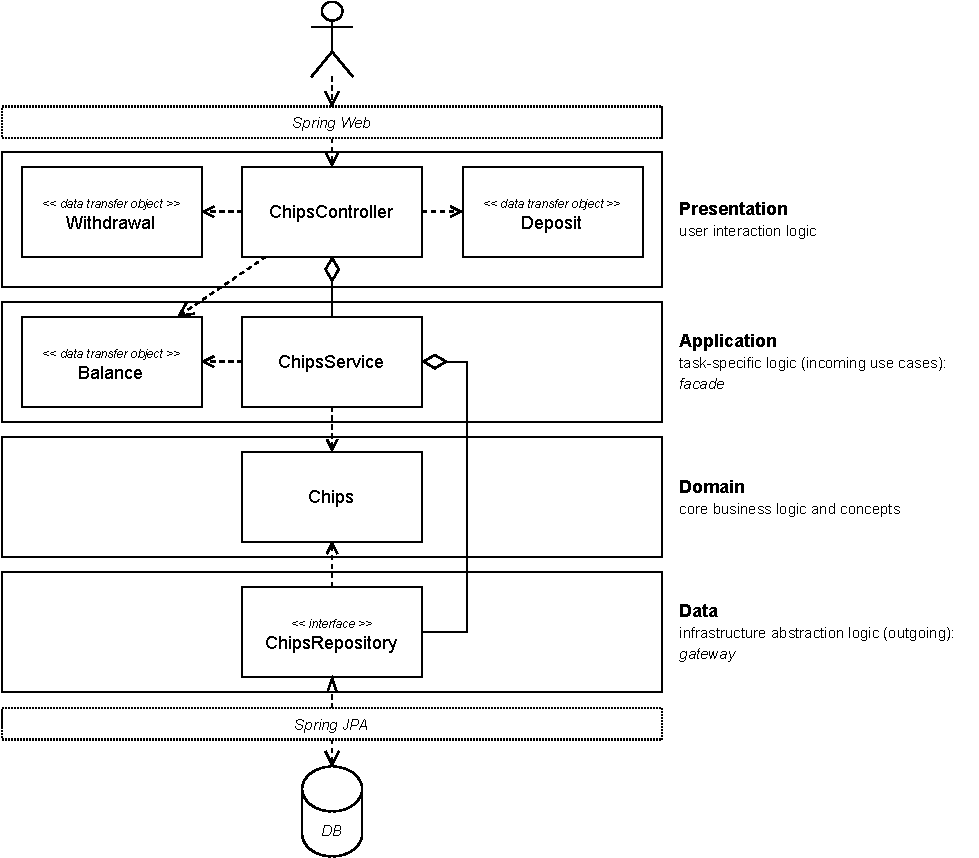
\includegraphics[width=0.8\linewidth]{chips-layers}
    \caption{De semi-gelaagde structuur binnen het chips-component.}
    \label{fig:chips-layers}
\end{figure}

\subsection{Applicatieflow}
Hoe loopt de flow binnen de de lagen in een component? 
Laten we daarvoor een blik werpen 
op de \emph{deposit use case} van het Chips-component.
Zie Figuur~\ref{fig:chips-sequence-diagram}.

\begin{figure}[H]
    \centering
    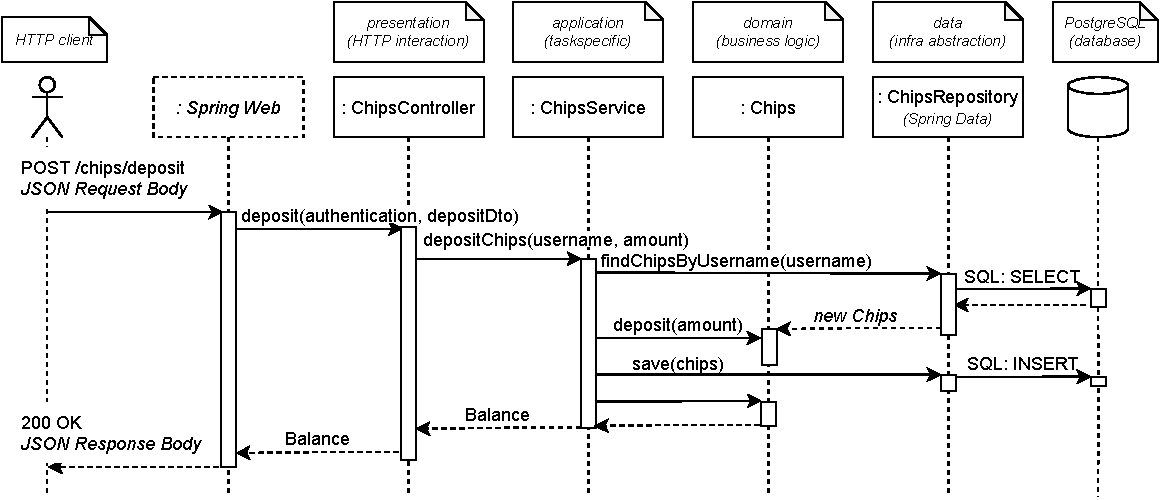
\includegraphics[width=\linewidth]{chips-sequence-diagram}
    \caption{De flow voor de deposit use case van het Chips-component}
    \label{fig:chips-sequence-diagram}
\end{figure}

Kijk ook in de code of je dit kunt herkennen!
Allereerst moet een HTTP-client een POST-verzoek doen naar 
\texttt{/chips/deposit}. We willen namelijk een overmaking toevoegen
aan de chips resource voor de huidige gebruiker. In dat POST-verzoek 
wordt de huidige gebruiker meegegeven via een JWT-token in de Authorization header
als deze is ingelogd. 

Vervolgens zet Spring Web dit verzoek om naar de bijbehorende 
controlleractie op de \emph{ChipsController} in de presentatielaag, met de
nodige informatie over de gebruiker (\emph{Authentication}) en de data die 
in de HTTP JSON Request Body zit (het \emph{Deposit} data transfer object).
De controller haalt de nodige data uit deze objecten en zet dit om naar 
een aanroep op de \emph{ChipsService} in de applicatielaag. 
Deze ChipsService bevat allerlei methoden die de use cases van 
het Chips-component vertegenwoordigen.
De service roept de \emph{ChipsRepository} aan uit de datalaag om de hoeveelheid
\emph{Chips} op te vragen voor de betreffende \emph{User} (op basis van de username). 
Vervolgens roept de service de \emph{deposit}-methode aan op de Chips om het aantal chips te verhogen met de 
gekozen hoeveelheid en wordt het \emph{Chips} object weer opgeslagen in de \emph{ChipsRepository}.
Ten slotte geeft de service een \emph{Balance} terug door de benodigde data uit het 
\emph{Chips}-object te halen en dit in een nieuw \emph{Balance}-object te stoppen.
De controller geeft ook deze \emph{Balance} terug aan Spring Web, waarop deze de 
\emph{Balance} omzet naar een HTTP JSON Response Body aan de hand van diens getters.

Voor het blackjack-component zou het ideaal zijn als wij ook één centraal object hebben 
om op te halen, domeinacties op uit te voeren en weer weg te schrijven. Het aan elkaar 
knopen daarvan kan gebeuren in use cases aangeboden in een BlackjackService!

\subsection{Frameworks}
Een \textit{framework} is code van anderen die je een hoop werk uit handen 
nemen ten aanzien van een of meer functionaliteiten. Het is een concrete, herbruikbare standaardoplossing.
Kenmerkend aan een framework is dat je als developer een deel van de controle 
uit handen geeft. Er is sprake van \textit{inversion of control}: het framework 
roept onze code aan op bepaalde plekken. Interactie met het framework vindt op twee plaatsen 
plaats:
\begin{enumerate}
    \item Entry points: hier roepen we het framework aan
    \item Hot spots: hier haken we onze eigen code in het framework en roept het framework onze code aan
\end{enumerate}

Er zijn twee soorten hot spots, die je kan herkennen vanuit het objectmodel:
\begin{enumerate}
    \item Composition hot spots: integratie van het aan een interface meegeven 
    van implementerende dependencies
    \item Inheritance hot spots: integratie via het overerven 
    van een vooropgezette klassenstructuur
\end{enumerate}

Beide vormen komen vaak voor in een framework.

In Spring herkennen we de \texttt{CasinoApplication} als entry point.
Deze is geannoteerd met \texttt{@SpringBootApplication}. Vervolgens laadt
Spring allerlei configuratie in, voert het een componentscan uit en klikt het dependencies in elkaar.
Spring's dependency injection is één van de composition hot spots die te vinden zijn in Spring,
terwijl Spring's repositories een vorm zijn inheritance hot spots.

\subsection{Dependency injection}
Dependency injection is niets anders dan het meegeven van afhankelijkheden,
in plaats van ze binnen de klasse aan te maken. Dit zorgt ervoor dat een klasse 
makkelijker uitbreidbaar en testbaar is. Hierover in een latere cursus meer.

In Spring maken we services aan door de klasse te annoteren met de \texttt{@Service} annotatie. 
We kunnen met dependency injection werken door de services (en opslagmechanismen) waarvan we afhankelijk zijn 
aan te geven in de constructor. Spring vindt dan automatisch welke services we bedoelen. 
Dit heet \textit{autowiring}.
Spring gaat tijdens een opstarten van de applicatie door onze code op zoek naar 
\texttt{@Bean}, \texttt{@Component}, \texttt{@Service}. Dit noem je Beans. 
Spring kijkt voor de dependencies naar de constructor en de benodigde interfaces 
en kijkt of er Beans zijn geconfigureerd die aan die interface voldoen. Met autowiring 
injecteert Spring de benodigde afhankelijkheid dus automatisch!

Kijk voor een voorbeeld wederom in het Chips-component.

Als alternatief voor constructor-injection kan 
je ook werken met de \texttt{@Autowired} annotatie 
op setters, constructor parameters of properties. 

Als we meerdere implementaties hebben van dezelfde interface 
(bijvoorbeeld omdat we een testimplementatie hebben), 
dan moeten we specifiek aangeven welke service we willen gebruiken. 
Dat kunnen we doen met de \texttt{@Qualifier} annotatie op zowel de service als binnen de constructor. 
Daarmee kwalificeren we om welke implementatieklasse het gaat door 
dit aan te geven boven elke \texttt{@Service} en vóór elke parameter in de 
constructor die de service gebruikt.

Met \texttt{@Value} kan je aangeven dat een waarde moet worden geïnjecteerd,
afkomstig is uit configuratie.

\section{Libraries}
Een library is ook een voorbeeld van een concrete, herbruikbare standaardoplossing.
Het belangrijkste verschil tussen een library en een framework is dat 
een framework veel meer controle opeist. Een library wordt door onze code aangeroepen
terwijl een framework uiteindelijk onze code aanroept (inversion of control).

Wel zie je vaak dat een framework gebruik maakt of zich openstelt voor verschillende
libraries door middel van composition hot spots. Vaak heb je dan een adapter nodig 
om de interface van het framework aan te passen aan de geboden facade van de library.
Dit zijn voorbeelden van design patterns. Hier gaan we het later uitgebreid over hebben.

\section{Stap 1: Maak een applicatieservice}
In ons domein hebben we een aantal domeinklassen gemaakt die verantwoordelijk 
zullen worden voor kleine acties per concept. Deze worden aan elkaar geknoopt 
door een dienstverlenend object dat verantwoordelijk is voor het omzetten van 
use cases naar domeinacties met behulp van infrastructuur. 
Dat wordt ook wel een \textit{application service} genoemd.

Maak eerst weer een package aan onder onze blackjack-component met de naam \texttt{application}
Dit is de applicatielaag waarin we onze taakgerichte logica (use cases) gaan uitvoeren.
Maak in die package een klasse aan: \texttt{BlackjackService}.
Het is immers een dienst die de acties aanbiedt om blackjack te kunnen spelen!
Deze wordt uiteindelijk aangesproken door de controller.

Vervolgens moeten we aan Spring doorgeven dat hij deze service kan gebruiken 
om te meegeven aan een andere service of bijvoorbeeld een controller als deze 
deze nodig heeft in de controller. Spring bevat een automatisch mechanisme 
voor \textit{dependency injection} en gebruikt daar annotaties voor. Om de service 
als zodanig vindbaar te maken, kan je \texttt{@Service} boven de klassedeclaratie plaatsen.

Dit zou er als volgt uit moeten zien:
\begin{minted}{java}
package nl.hu.bep2.casino.blackjack.application;

@Service
public class BlackjackService {
}
\end{minted}

\section{Stap 2: Bedenk welke methodes we nodig hebben}
Welke acties moet onze service aanbieden? 
Dit komt overeen met de use cases van onze component! 
Als het goed is, hebben we hiervoor een use case diagram gemaakt.

Maak public methods aan met de namen van deze use cases volgens 
de naming conventions van Java (\textit{camelCase}). 
Bedenk per methode ook wat voor een input we nodig hebben.
Voor sommige methoden is het handig om het spel te kunnen identificeren
op basis van een id (type: \textit{Long}). Voor de meeste methoden hebben 
we daarnaast de naam van de gebruiker nodig (type: \textit{String}).

De identifier zullen we automatisch door de database laten genereren
zodra we met persistentie bezig gaan.

\subsection{Voorbeeld: Het starten van het spel}
Laten we als voorbeeld het starten van een spel als use case nemen.
Het is belangrijk om hier een duidelijke, beschrijvende naam voor te pakken,
bijvoorbeeld: \textit{startGame} of \textit{start}.

\subsubsection{Method arguments}
Wat moeten we allemaal meegeven als parameters om het spel te starten?

Om het spel te kunnen opzoeken voor deze speler is het handig om de naam van de speler  
te bewaren. We kunnen een parameter toevoegen met als type \texttt{String} en 
als naam \texttt{playerName}. 
Omdat een speler meerdere spellen kan hebben, moeten we ervoor zorgen 
dat de database ook elk spel voorziet van een unieke identifier. 
Dat doen we later wanneer we met persistentie bezig gaan.

Het is handig om het spel meteen te beginnen met een inleg. Dat bespaart ons een
extra HTTP request! Laten we de parameter \texttt{Integer bet} toevoegen.

Meer hebben we niet nodig van de speler!

\subsubsection{Return type}
Wat willen we teruggeven nadat we het spel hebben gestart? 
Hier kunnen we wat slims verzinnen om aan de speler te laten zien hoe 
het spel er nu uitziet: de spelvoortgang. 
We willen uiteindelijk namelijk in de controller
een bericht terugsturen naar de HTTP client met daarin een JSON body 
met alle informatie. Een front-endprogrammeur kan dat mooi weergeven met
afbeeldingen en interacties.

Welke informatie willen we aan de speler laten zien
en hoe kunnen we dat het best structureren? Dat laten we aan jou over!
Alvast een tip: we kunnen een String teruggeven, 
maar dan gaat er een boel gestructureerde informatie verloren!

\subsection{Stap 3: Vul de methodes in}
Nadat we bedacht hebben welke methodes onze service moet hebben, 
kunnen we naar de invulling van die methodes kijken.
Het is het mooiste als applicatieservices niet teveel logica bevatten,
maar het gros van het werk door domeinobjecten wordt gedaan.
Op deze manier houd je een abstract en herbruikbaar domein en is je 
applicatieservice een soort samenvatting van hoe het domein zich gedraagt.

Probeer in algemene bewoordingen de acties te beschrijven 
en gaandeweg acties toe te voegen aan de centrale domeinentiteit
en de domeinobjecten die daarin gebruikt worden.

\subsubsection{Voorbeeld: Method body van startGame}
We hebben een methodenaam, parameters en een return type gedeclareerd.
Welke stappen willen we uitvoeren in de methode? 

Globaal zal je op de volgende zaken uitkomen:

\begin{enumerate}
    \item Neem het aantal chips op ter hoogte van de bet
    \item Maak een nieuw spel aan
    \item Start het spel
    \item Sla het spel op
    \item Stort chips als sprake van blackjack of push
    \item Geef de voortgang terug
\end{enumerate}

Voor het starten van het spel kan je een methode op het Game object maken,
genaamd \textit{start}. Je kan ervoor kiezen om de benodigde parameters mee te geven aan de 
constructor of de start methode. Wat deze methode moet doen laten we aan jou over.
Een aantal tips: wat moet de speltoestand zijn bij het beginnen van het spel?
Laat je het spel zelf een nieuwe Deck maken of doen we dat in de application service?

Bij de uitvoering van \textit{game.start()}, maken we onder andere gebruik van 
Deck en vast ook wel van andere klassen en enums! 
De kaarten moeten worden geschud en op de hand worden gebracht van de speler 
en van de dealer. Vervolgens moeten scores berekend worden en de huidige speltoestand 
geupdatet worden.

Het opslaan van het spel kan je nog even laten zitten,
maar het is misschien handiger om dit tijdelijk te doen 
door een field op te nemen in de application service.
Je zou hiervoor een \texttt{Map<String, Game>} kunnen gebruiken 
waarmee tijdelijk spellen (\textit{value}) bewaard kunnen worden 
op basis van spelernaam (\textit{key}).

Dit gaan we in een van de volgende opdrachten vervangen met apart object dat verantwoordelijk 
is voor de langdurige opslag van spellen: een GameRepository.

\subsubsection{Bescherm in domeinacties tegen ongeldige situaties (invariants)}
Je domein bepaalt hoe de regels van de kernconcepten eruit zien.
Bij een spel zijn het bijvoorbeeld letterlijk de spelregels.
Zie bijvoorbeeld de Chips-klasse: je mag geen negatieve hoeveelheid opnemen 
en je mag geen chips opnemen als je saldo te laag is.

\begin{minted}{java}
 public void withdraw(Long amountToWithdraw) {
    if (amountToWithdraw < 0) {
        throw new NegativeNumberException("Cannot withdraw a negative amount: " + amountToWithdraw);
    }

    long newAmount = this.amount - amountToWithdraw;
    if (newAmount < 0) {
        throw new NotEnoughChipsException(
                String.format(
                        "Cannot withdraw %d chips: %d chips remaining",
                        amountToWithdraw,
                        this.amount
                )
        );
    }

    this.amount = newAmount;
}    
\end{minted}

Voor het spelen van het spel geldt hetzelfde. Je mag natuurlijk 
geen zetten doen als het spel is afgelopen! Hiervoor kan je een \textit{guard-clause} gebruiken:
een \textit{if-statement} die een exception gooit als iets niet mag. Je hebt geen \textit{else} nodig! 
De flow wordt immers doorbroken als er sprake is van een exception.

\subsubsection{Overige use cases en domeinacties}
Doe hetzelfde voor de overige use cases en domeinacties. 
Hier gaat een boel tijd inzitten, 
dus het is niet erg als je dit later verbetert wanneer we 
de persistentie en de web API ingericht hebben.

Commit je wijzigingen met een duidelijke naam, 
bijvoorbeeld: "Add use cases to blackjack service". 
Push de wijzigingen naar je remote GitHub repository.
\documentclass[dutch,a4paper,12pt,doubleside]{book}

\usepackage[T1]{fontenc}
\usepackage[dutch]{babel}
\usepackage[utf8]{inputenc}
\usepackage[margin=3cm]{geometry}
\usepackage{amsthm}
\usepackage{hyperref}
\usepackage{minted}
\usepackage{float}
\usepackage{trimspaces}
\usepackage[nottoc]{tocbibind}
\usepackage[labelfont=bf]{caption}
\usepackage{tabularx}
\usepackage{array}
\usepackage{dirtree}

% headers and footers (page numbering)
\usepackage{fancyhdr}
\fancyhf{} % clear all header and footers
\renewcommand{\headrulewidth}{0pt} % remove the header rule
\fancyfoot[R]{\thepage} % Left side on Even pages; Right side on Odd pages
\pagestyle{fancy}
\fancypagestyle{plain}{%
  \fancyhf{}%
  \renewcommand{\headrulewidth}{0pt}%
  \fancyhf[lef,rof]{\thepage}%
}

% Card suits
\DeclareSymbolFont{extraup}{U}{zavm}{m}{n}
\DeclareMathSymbol{\varheart}{\mathalpha}{extraup}{86}
\DeclareMathSymbol{\vardiamond}{\mathalpha}{extraup}{87}

\usepackage{makeidx}
\usepackage{hyperref}
\usepackage{minted}

% New line per paragraph, instead of indentation
\usepackage[parfill]{parskip}

% Prevent balancing vertical alignment
\raggedbottom

% Sets global font
\usepackage{tgpagella}

% Font utility function
\newcommand{\fon}[1]{\fontfamily{#1}\selectfont}

\usepackage[table, x11names]{xcolor}
\definecolor{blue}{RGB}{0, 149, 200}
\definecolor{green}{RGB}{0, 200, 136}

\captionsetup{justification=raggedright,width=.8\linewidth}

\usepackage[many]{tcolorbox}
\newtcolorbox{deftbox}{
    enhanced,
    sharp corners,
    frame hidden,
    boxrule=0em,
    left=1em,
    toptitle=1em,
    top=0.25em,
    bottom=1em,
    bottomtitle=0mm,
    colback=black!4,
    colbacktitle=black!4,
    coltitle=black!60,
    fonttitle=\bfseries\small,
    fontupper=\small,
    borderline west={2pt}{0pt}{black!20},
    grow to left by=-2em,
    grow to right by=-2em
}
\newtcolorbox{defbox}[1]{
    enhanced,
    sharp corners,
    frame hidden,
    boxrule=0em,
    left=1em,
    toptitle=1em,
    top=0.25em,
    bottom=1em,
    bottomtitle=0mm,
    colback=black!4,
    colbacktitle=black!4,
    coltitle=black!60,
    fonttitle=\bfseries\small,
    fontupper=\small,
    borderline west={2pt}{0pt}{black!20},
    grow to left by=-2em,
    grow to right by=-2em,
    title={#1}
}
\newtcolorbox{quotebox}{
    enhanced,
    sharp corners,
    frame hidden,
    left=1em,
    right=1em,
    top=1em,
    bottom=1em,
    colback=black!4!white,
    fontupper=\small,
    grow to left by=-2em,
    grow to right by=-2em
}

\def\trim#1{\ignorespaces#1\unskip}

\newcommand{\blockquote}[2]{
    \hfill
    \begin{quotebox}
    \begin{flushleft}
        ``\trim{#1}''
        \newline\newline\rightline{\textbf{-- \trim{#2}}}
    \end{flushleft}
    \end{quotebox}
    \noindent
}

\renewcommand{\listingscaption}{Codevoorbeeld}
\renewcommand{\listoflistingscaption}{Overzicht van codevoorbeelden}
\counterwithin{listing}{chapter}
% \usepackage[chapter]{minted}



\begin{document}

\setcounter{chapter}{3}
\chapter{Opdracht 4: Web API}
Onze applicatie presenteert zichzelf naar buiten toe via het web:
we reageren op HTTP requests en geven HTTP responses terug.

\section{Client/server-architectuur}
Het web werkt volgens een client/server-architectuur (of klant/bediende-model):
We hebben een client, bijvoorbeeld een web browser, die een verzoek doet 
aan een server die dit afhandelt. Zie Figuur~\ref{fig:client-server}.

\begin{figure}[H]
    \centering
    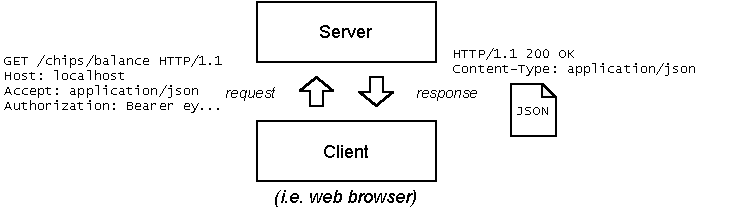
\includegraphics[width=.9\linewidth]{client-server}
    \caption{HTTP requests worden van een client gestuurd naar een server, welke dit verwerkt en reageert met een HTTP response.}
    \label{fig:client-server}
\end{figure}

\section{Content negotiation}
Zoals in Figuur~\ref{fig:client-server} is te zien, 
onderhandelen client en server over het ophalen van een \textit{representatie}
van een bepaalde \textit{resource}. We zien dat de client een 
GET-verzoek doet naar localhost voor een Balance-resource te
vinden via de Uniform Resource Locator (URL) `chips/balance'
(in combinatie met de token in de Authorization header)
De gewenste representatie daarvan moet `application/json' zijn.

Deze interactie tussen client en server noem je \texit{content negotation}:
er is een scheiding tussen de abstractie en de verschijningsvorm ervan.

\section{HTTP requests}
Een HTTP request (zie Figuur~\ref{fig:client-server}) wordt gevormd door:
\begin{enumerate}
    \item Een beschrijving van method, URI en protocol
    \item Headers
    \item Optioneel: een request body met een representatie volgens Content-Type
\end{enumerate}

\subsection{HTTP methods}
De HTTP-specificatie beschrijft een aantal methodes 
waarmee een client allerlei zaken kan vragen aan een server.
Het is belangrijk om de juiste HTTP-methodes te gebruiken omdat 
deze in de eerste plaats het soort actie aangeven die wordt verzocht.

In de tweede plaats staat in de protocol-specificatie van HTTP heel 
nauwkeurig beschreven wat clients en servers mogen verwachten van een 
bepaalde HTTP-methodes. 
Twee van de te verwachten eigenschappen zijn \textit{safety}
en \textit{idempotentie}.

Een HTTP-method wordt als \textit{safe} beschouwt als deze niet 
de intentie heeft om de servertoestand aan te passen. 
Dat betekent dat het gaat om read-only methoden. Safe 
methoden kunnen helpen bij het cachen van resultaten (zie: REST).
Bij safety gaat het dus niet om de beveiliging, het ziet 
erop dat het veilig is omdat het geen toestand kan aanpassen.

Wanneer een HTTP-method \textit{idempotent} wordt genoemd,
betekent dat dat we het verzoek meerdere keren kunnen herhalen
zonder dat de uitkomst op server verandert. Denk bijvoorbeeld aan 
het tweemaal uitvoeren van een \texttt{DELETE}-methode. Beide keren is 
de betreffende resource verwijderd. Idempotentie helpt een API betrouwbaar 
te maken tegen fouten: het betekent dat je een verzoek kan herhalen zonder 
als je als client niet zeker weet of het is aangekomen of niet.

We kennen de volgende HTTP-methods, zie Figuur~\ref{table:http-methods}:

\begin{table}[H]
\centering
\begin{tabularx}{\textwidth}{
    |>{\raggedright}l|>{\raggedright}X|>{\raggedright}X|>{\raggedright\arraybackslash}X|
}
\hline
\textbf{Method} & \textbf{Bedoeling} & \textbf{Safe} & \textbf{Idempotent} \\ \hline
\texttt{GET} & opvragen van resource(s) & Ja & Ja \\ \hline
\texttt{HEAD} & opvragen van headers (voordat je een mogelijk grote GET-request doet) & Ja & Ja \\ \hline
\texttt{OPTIONS} & opvragen van toegestane communicatiewijzen voor een bepaalde URL of server & Ja & Ja \\ \hline
\texttt{TRACE} & opvragen van afgelegde weg van het verzoek ter debugging & Ja & Ja \\ \hline
\texttt{DELETE} & verwijderen van gehele resource op basis van URL (met identifier) & Nee & Ja \\ \hline
\texttt{PUT} & aanmaken/wijzigen van gehele resource op basis van URL (met identifier) & Nee & Ja \\ \hline
\texttt{PATCH} & wijzigen van deel van resource op basis van URL (met identifier) & Nee & Nee \\ \hline
\texttt{POST} & aanmaken nieuwe resource op onder een bepaalde URL (zonder identifier) & Nee & Nee \\ \hline
\end{tabularx}
\caption{Een opsomming van HTTP-methoden, hun bedoeling en verwachte eigenschappen}
\label{table:http-methods}
\centering
\end{table}

\newpage
\section{HTTP responses}
Een HTTP response (zie Figuur~\ref{fig:client-server}) wordt gevormd door:
\begin{enumerate}
    \item Een beschrijving van protocol en statuscode
    \item Headers
    \item Optioneel: response body met een representatie volgens Content-Type 
\end{enumerate}

\subsection{Status codes}
Het teruggeven van de juiste statuscode is erg belangrijk wanneer je een API 
ontwerpt. Het maakt een bepaalde verwachting duidelijk en clients krijgen zo 
de mogelijkheid om slim om te gaan als er bijvoorbeeld een redirection moet plaatsvinden
of als de client wat verkeerd heeft gedaan.

HTTP status codes worden onderverdeeld 5 categorieën, waarbij 
het eerste getal steeds de categorie aangeeft (we noemen er hier een paar):
\begin{itemize}
    \item \textbf{1xx Informational}: request ontvangen, verwerking gaat door
        \begin{itemize}
            \item \textbf{100 Continue}: wordt gebruikt als een client eerst wil checken of de server het verzoek 
            gaat accepteren, bijvoorbeeld bij grote request bodies.
        \end{itemize}
    \item \textbf{2xx Successful}: request ontvangen, begrepen, en geaccepteerd zonder problemen
        \begin{itemize}
            \item \textbf{200 OK}: standaardresponse voor succesvolle afhandeling
            \item \textbf{201 Created}: verzoek is afgehandeld; een resource is succesvol aangemaakt
            \item \textbf{202 Accepted}: verzoek is succesvol binnengekomen, maar de uitvoering volgt nog
        \end{itemize}
    \item \textbf{3xx Redirection}: meer actie is vereist om het verzoek af te handelen
    \begin{itemize}
        \item \textbf{303 See Other}: de response voor het request kan worden opgehaald (met GET) via de getoonde URI
        \item \textbf{307 Temporary Redirect}: dit verzoek, niet volgende verzoeken, moet worden herhaald naar een andere URI (met dezelfde method)
        \item \textbf{308 Permanent Redirect}: dit verzoek en volgende verzoeken moeten worden herhaald naar een andere URI (met dezelfde method)
    \end{itemize}
    \item \textbf{4xx Client Error}: de client heeft iets fout gedaan bij het doen van het verzoek
    \begin{itemize}
        \item \textbf{400 Bad Request}: algemene fout om aan te geven dat het request van de client niet klopt
        \item \textbf{401 Unauthorized}: lijkt op 403, maar client moet zich authenticeren
        \item \textbf{402 Payment Required}: er moet betaald worden om de request af te handelen (wordt weinig gebruikt)
        \item \textbf{403 Forbidden}: client heeft geen toestemming om de request te laten afhandelen
        \item \textbf{404 Not Found}: resource kan niet gevonden worden
        \item \textbf{405 Method not Allowed}: de betreffende HTTP-methode mag niet worden uitgevoerd
        \item \textbf{406 Not Acceptable}: de gespecificeerde Content-Type kan niet afgehandeld worden
    \end{itemize}
    \item \textbf{5xx Server Error}: het verzoek lijkt er goed uit te zien, maar er gaat iets fout op de server
    \begin{itemize}
        \item \textbf{500 Internal Server Error}: algemene fout om aan te geven dat er iets fout is gegaan op de server
        \item \textbf{502 Bad Gateway}: de server gaf de afhandeling door aan een ander systeem, maar daar gaat iets fout
        \item \textbf{503 Service Unavailable}: de server kan het verzoek niet afhandelen vanwege onderhoud of drukte
    \end{itemize}
\end{itemize}

Deze statuscodes zijn als enum opgenomen in Spring, te vinden in 
\href{https://docs.spring.io/spring-framework/docs/current/javadoc-api/org/springframework/http/HttpStatus.html}{\texttt{HttpStatus}}.
Standaard geeft Spring een \texttt{200 OK} terug als het een object in de controller teruggeeft
en een \texttt{500 Server Error} als er iets fout gaat bij de verwerking.

\section{Representational State Transfer (REST)}
\textit{Representational State Transfer (REST)} is een architecturele stijl,
een set aan afspraken om een aantal problemen van het vroege web op te lossen.
Het is een standaard die door de meeste webapplicaties,
bewust of onbewust, wordt toegepast.

Deze eigenschappen en aanbevelingen zijn beschreven in de baanbrekende 
PhD-thesis van Roy Fielding.

Er zijn een aantal eigenschappen waar REST een oplossing voor wil 
bieden:
\begin{itemize}
    \item performance in de communicatie tussen componenten
    \item schaalbaarheid van componenten en interactie ertussen
    \item een eenvoudige, voorspelbare interface (API)
    \item aanpasbaarheid van componenten
    \item zichtbaarheid van communicatie tussen componenten
    \item portabiliteit van componenten door het versturen van data te verrijken met code (JavaScript)
    \item betrouwbaarheid bij foutafhandeling binnen en tussen componenten
\end{itemize}

Deze eisen hebben geleid tot zes architecturele \textit{constraints} (beperkingen):

\subsection{Client/server}
Een scheiding van client en server leidt tot \textit{separation of concerns} en 
zorgt voor portabiliteit. Een server kan verschillende soorten clients bedienen.

\subsection{Stateless communicatie}
Client-servercommunicatie moet stateless zijn. 
Dat betekent dat alle benodigde informatie om het request af te handelen in het request (url, headers, body) moet zijn opgenomen.

Dit brengt een hoop voordelen met zich mee. Dit leidt tot schaalbaarheid
van servers. Het maakt niet uit welke fysieke server het request afhandelt,
omdat er alle benodigde informatie in de request zit. Zo kan je honderden (virtuele) 
servers neerzetten met dezelfde code om overbelasting te voorkomen.
Tegenwoordig zie je de grootste performance-problemen ontstaan in de 
inrichting van de persistentie. Dit is lastig op te schalen, 
omdat de application state ergens moet leven.

Het maakt het ook makkelijker voor servers om te herstellen van fouten.
Het request kan immers gewoon volledig ge-retried worden door de client.

Ten slotte zijn requests over het algemeen makkelijker af te handelen 
omdat de server niet hoeft bij te houden waar elke client zich bevindt 
in het systeem en welke informatie voor een bepaalde sessie nog onthouden 
moet worden. Dat moet de client allemaal doen.

Session state moet dus op de client bewaard worden, 
bijvoorbeeld met een local storage.
Wij sturen dan ook steeds de session state 
mee in de JWT-token in de Authorization header.
De Postman-collectie zorgt ervoor dat dit automatisch gebeurt.

\subsection{Cacheability}
Om de netwerk-efficiëntie nog meer te vergroten, moeten we slim 
omgaan met caching. Een \textit{cache} zorgt ervoor dat we niet 
het verzoek nogmaal in zijn volledigheid hoeven te verwerken,
maar dat we het resultaat van eenzelfde eerdere request 
kunnen teruggeven. Dat is wel zo snel.

Caching is in de praktijk erg moeilijk om te regelen. Daarom 
zijn er op het gebied van HTTP en REST een aantal afspraken ten 
aanzien van het soort \textit{request methods} die veilig zijn 
om te gebruiken of niet.

\subsection{Uniform interface}
We kennen het ontwerpprincipe dat we willen programmeren tegen 
standaardabstracties (\textit{program to an interface}), zodat 
de onderliggende implementatie kan variëren. Om een gestandaardiseerde 
interface te behouden, moeten we rekening houden met:
\begin{enumerate}
    \item Uniform Resource Identifiers (URIs)
    \item manipuleren van resources via representaties
    \item self-descriptive messages
    \item Hypermedia As The Engine Of Application State (HATEOAS)
\end{enumerate}

Voor de uniform interface is het belangrijk 
om in de URL te werken met identificeerbare 
resources! Stop geen acties in de URL, maar gebruik
daar de HTTP-methodes voor. Denk niet in termen van uitvoering,
maar in termen van het aanmaken, verwijderen of wijzigen van 
resources door een representatie van die resource te sturen. 

In het ideale geval zit alle informatie in de response ingebakken,
ook welke acties nog meer mogelijk zijn met de betreffende resource.
Dat is wat HATEOAS inhoudt.

\subsection{Layered system}
Clients zouden alleen maar weet moeten hebben van één server 
om een bepaalde resource op te vragen of te bewerken. Dat er 
op de achtergrond allerlei andere systemen spelen zou niet relevant 
moeten zijn. Dit zorgt ervoor dat de client kan koppelen tegen 
een centrale API (ook wel een API-gateway) genoemd, terwijl er op 
de achtergrond allerlei wijzigingen en optimalisaties plaats kunnen
vinden. Caching kan worden toegevoegd, de dataopslag kan slimmer 
ingericht worden, hele back-ends kunnen worden herschreven: de client 
hoeft hier (wat de API betreft) weinig van te merken.
Dit is \textit{high cohesion} 
en \textit{loose coupling} op HTTP niveau!

\subsection{Code-on-demand (optional)}
Binnen REST kunnen we de mogelijkheid aan servers bieden om gedrag 
op de client uit te breiden. Het eerste verzoek aan een server geeft 
meestal een hele set aan JavaScript terug om zo de gebruikerservaring 
te verrijken!

Een RESTful systeem moet zo zijn opgezet dat dit mogelijk is.

\subsection{RESTful of niet?}
Striktgenomen noemen we een web service RESTful als deze voldoet aan 
alle principes van REST. In de praktijk is dat helaas niet het geval
en worden veel web APIs RESTful genoemd zonder dat aan alle voorwaarden 
wordt voldaan.

\section{Stap 1: Ontwerp de web API op basis van REST}
Als we volgens REST met HTTP willen werken, bieden we meestal per resource een endpoint aan. 
REST is een gestandaardiseerde manier van werken. 
Het is de moeite waard om te kijken of we dit op de juiste manier implementeren. 
Niet alleen omdat we erop beoordeeld worden, maar ook omdat men in de praktijk bepaalde verwachtingen heeft van een REST API.

We moeten in het kader van de uniform interface rekening houden met:
\begin{enumerate}
    \item De juiste URL-structuur
    \item De juiste HTTP-request methods en headers
    \item De juiste parameters in URL, query en body
    \item De juiste HTTP-response codes, headers en body
\end{enumerate}

Via content negotiation wordt binnen REST een representation 
aangeboden van de resource, zoals bijvoorbeeld JSON of XML. 
Met de \textit{Accept header} kunnen client en server aangeven 
met welke representation kan worden gewerkt. 
Met de \textit{Content-Type header} kan worden aangegeven 
welk soort representation in de body van de request of de response is opgenomen.

Ontwerp hoe je web API eruit moet komen te zien.

Je mag dit documenteren in je project,
bijvoorbeeld in een \textit{web-api.md}, maar dat hoeft niet.
Als voorbeeld kan je hiernaar kijken (voor de web API van chips, zie de ChipsController).
\begin{minted}{markdown}
# Chips API

## Show balance: hoeveel chips bekijken
Route: `GET /chips/balance`
Response body: JSON met chips in account

## Withdraw chips: een "withdrawal" toevoegen
Route: `POST /chips/withdrawal`
Request Body: JSON met chips om op te nemen
Response body: JSON met chips in account

## Deposit chips: een "deposit" toevoegen
Route: `POST /chips/deposit`
Request Body: JSON met chips om te storten
Response body: JSON met chips in account

## Status codes
* 200 OK: alles goed gaat
* 400 Bad Request: gebruiker geeft foutieve invoer (bijvoorbeeld: negatief aantal)
* 401 Unauthorized: gebruiker is niet ingelogd 
* 402 Payment Required: gebruiker heeft niet genoeg chips
\end{minted}

\section{Stap 2: Implementeer de API met Spring Boot}
Spring Boot maakt gebruik van de Spring Web MVC library om web requests
af te handelen via controllers. 
Intern wordt er gebruikt gemaakt van een embedded Tomcat-instantie,
zodat we niet met losse WAR-bestanden en Java application containers aan de slag hoeven.

Hier volgt een overzicht van hoe je dingen kan aanpakken in 
Spring Boot, maar kijk ook eens in het chips-component!
Daar wordt al een boel uit duidelijk. Voor meer informatie, zie:
\href{https://docs.spring.io/spring-framework/docs/5.3.8/reference/html/web.html#mvc-controller}{De Spring Web MVC documentatie}.

\begin{minted}{java}
@RestController
@RequestMapping("/chips")
public class ChipsController {
    private final ChipsService service;

    public ChipsController(ChipsService service) {
        this.service = service;
    }

    @GetMapping("/balance")
    public Balance showBalance(Authentication authentication) {
        UserProfile profile = (UserProfile) authentication.getPrincipal();
        Balance balance = this.service.findBalance(profile.getUsername());

        return balance;
    }

    @PostMapping("/deposit")
    public Balance deposit(Authentication authentication, @Validated @RequestBody Deposit deposit) {
        UserProfile profile = (UserProfile) authentication.getPrincipal();

        try {
            Balance balance = this.service.depositChips(profile.getUsername(), deposit.amount);
            return balance;
        } catch (NegativeNumberException exception) {
            throw new ResponseStatusException(HttpStatus.BAD_REQUEST, exception.getMessage());
        }
    }

    @PostMapping("/withdrawal")
    public Balance withdraw(Authentication authentication, @Validated @RequestBody Withdrawal withdrawal) {
        UserProfile profile = (UserProfile) authentication.getPrincipal();

        try {
            Balance balance = this.service.withdrawChips(profile.getUsername(), withdrawal.amount);
            return balance;
        } catch (NotEnoughChipsException exception) {
            throw new ResponseStatusException(HttpStatus.PAYMENT_REQUIRED, exception.getMessage());
        } catch (NegativeNumberException exception) {
            throw new ResponseStatusException(HttpStatus.BAD_REQUEST, exception.getMessage());
        }
    }
}
\end{minted}

Het is de verantwoordelijkheid van een controller om een HTTP-request
om te zetten naar Java-code, een use case uit te voeren op een service, 
en het resultaat weer om te zetten naar een HTTP-response. 
Controllers zijn onderdeel van de presentatielaag omdat 
het één van de manieren is waarmee een component zijn diensten kan aanbieden 
aan de buitenwereld. We zouden bijvoorbeeld ook commandline commands kunnen maken 
die precies dezelfde use cases moeten kunnen uitvoeren. Die kunnen dan gebruik 
maken van exact dezelfde applicatielaag!

Implementeer de web API voor ons blackjack-component. Houdt rekening met 
de correcte URLs, HTTP methods en HTTP statuscodes. Werk natuurlijk 
je application services en domeinacties bij om ze verder werkend te krijgen.

Test je applicatie uit met Postman.
Vergeet niet om de aangemaakte endpoints ook 
in je Postman-collectie aan te maken, 
zodat authenticatie en autorisatie automatisch 
gaan via de bij het inloggen verkregen JWT-token!

Commit je wijzigingen met een duidelijke naam, 
bijvoorbeeld: "Add blackjack web API". 
Push de wijzigingen naar je remote GitHub repository.

Hier volgt wat meer informatie om je op weg te helpen.

\subsection{Controller: \texttt{@RestController}}
In Spring Boot maken we een controller door de klasse te annoteren 
met \texttt{@RestController}. Hiermee wordt aan Spring doorgegeven
dat de verschillende routes (request mappings) moeten worden verzameld
en dat de controller gebruik kan maken van dependency injection.

\subsection{Resources en routes: \texttt{@RequestMapping}}
In Spring kan je een HTTP resource aangeven door boven een controller
de annotatie \texttt{@RequestMapping} toe te voegen. In deze annotatie 
kan je een pad meegeven om aan te geven wat het hoofdpad is voor deze controller.
Dit komt vaak overeen met de component-naam, de naam van de centrale entiteit of beide.

Per Java-methode kunnen we ook request mappings toevoegen. We kunnen zelfs specificeren
om wat voor een soort request-method het gaat door dat te specificeren.
\texttt{@PostMapping("/deposit")} leidt bijvoorbeeld tot de route `/chips/deposit' op 
de host. Op onze ontwikkelomgeving is de host `localhost:8080'.

Aan een RequestMapping kan je ook nog allerlei extra waarden meegeven, waaronder 
de content-types die ondersteund worden en de content-types die kunnen worden teruggegeven.
Standaard accepteert en stuurt Spring Boot JSON. We hoeven dus niets in te stellen.

\subsection{Data uit URL: \texttt{@PathVariable}}
In een URL wil je het mogelijk maken om een bepaalde resource te vinden. 
Je wil een identifier (id) mee kunnen sturen.
Met \texttt{@PathVariable} kunnen we data uit een URL halen. Deze annotatie zet je voor 
de argumenten van de Java-methode. De naam van het argument moet overeenkomen met de naam 
in het pad. Stel dat we een methode willen 
maken die een Game kan ophalen 
(of eigenlijk: de voortgang van het spel, we willen geen hole-card tonen), 
dan zou dat er als volgt uit kunnen zien:
\begin{minted}{java}
    @GetMapping("/{id}")
    public Game findGame(Authentication authentication, @PathVariable id) {
        UserProfile profile = (UserProfile) authentication.getPrincipal();
        GameProgress progress = this.blackjackService.findGame(profile.getUsername(), id);
        return progress;
    }
}
\end{minted}

\subsection{Data uit request body (DTO): \texttt{@RequestBody}}
In een aantal gevallen wil de client data meesturen maar de server, zoals 
bijvoorbeeld bij een \texttt{POST}, \texttt{PATCH} of \texttt{PUT}. 
Dit doe je in de request body. In Spring maken we hiervoor een simpel
data transfer object (DTO) met ofwel getters en setters, ofwel publieke velden. 
Zie bijvoorbeeld de deposit-methode van de Chips-controller.
Hierin wordt gebruik gemaakt van een Deposit-klasse waarin een aantal is
opgenomen:

\begin{minted}{java}
    // nl.hu.bep2.casino.chips.controller.ChipsController.java
    @PostMapping("/deposit")
    public Balance deposit(Authentication authentication, @Validated @RequestBody Deposit deposit) {
        // ...
    }

    // nl.hu.bep2.casino.chips.dto.Deposit.java
    public class Deposit {
        @Positive
        public Long amount;
    }
\end{minted}

Een leuke extra is dat je in Spring ook validatie kan toevoegen.
Dan voeg je een \texttt{@Validated}-annotatie toe aan de method-argument in de controller
en kan je verschillende validators toepassen op de velden in de DTO.

Wanneer de gebruikersinvoer niet klopt, geeft Spring automatisch 
een \texttt{400 Bad Request} terug met een foutmelding!
Merk op dat we deze check zowel in het domein uitvoeren als in de presentatielaag.
Dit heet \textit{defense-in-depth}: we garanderen dat het domein altijd klopt,
maar checken op meerdere plekken om zo vroeg mogelijk feedback te geven. 

\subsection{Data uit query parameters: \texttt{@RequestParam}}
Waarschijnlijk niet van toepsing op ons project,
maar je kan in een URL ook query parameters toevoegen.
Dit ziet er vaak uit als een reeks keys en values achter een vraagteken,
vaak om een bepaalde verzameling aan resultaten te filteren of ordenen:
\texttt{GET /search?q=cohesion\&src=typed\_query} met als host \textit{twitter.com} 
toont de tweets die voldoen aan de zoekquery ``cohesion''.

We kunnen een dergelijke variabele inzetten op dezelfde manier als we doen voor 
een \texttt{@PathVariable}, alleen hoef je niets aan te geven in de 
requestmapping-route. Voor ons project zullen we dit niet per se nodig hebben.

\subsection{JSON-serializatie}
We hoeven in een controller niets meer om te zetten en kunnen een object 
teruggeven. Spring verzorgt een automatische serializatie van een object naar JSON
op basis van de getters van het betreffende object (en de getters van alle objecten daarbinnen).
Hetzelfde geldt voor publieke velden. Ook deze worden automatisch omgezet.

Standaard wordt er dan een \texttt{200 OK} terug gegegeven.
Wil je meer controle dan kan je kijken naar \texttt{ResponseEntity}
en \texttt{@ResponseStatus}.

Let wel op dat je hiermee extra getters toevoegt in je \textit{domeinlaag}, alleen maar 
om een JSON-veld toe te voegen in je \textit{presentatielaag}. Dit introduceert (indirecte)
coupling. Voor dit project is dat niet erg. Mocht je verder willen ontkoppelen, dan kan je 
in je applicatielaag een vertalingsslag maken van domeinobjecten naar DTOs die een bepaald 
resultaat vertegenwoordigen.

\subsection{Pro-tip: Foutafhandeling}
Spring handelt standaard alle ongespecificeerde fouten af met een 500.

Voor custom foutafhandeling kan je werken met een \texttt{try/catch}. 
Op die manier kan je (domein-)excepties omzetten naar
\texttt{ResponseException}s. Daar kan Spring foutberichten van maken.
Zie hiervoor ook de ChipsController.

Wil je een slimmere manier om foutafhandeling te regelen? Dan kan je 
kijken naar \texttt{@ControllerAdvice} of \texttt{@ExceptionHandler}.
\textit{Google is your friend!}

\end{document}
\chapter{Opdracht 5: Persistentie}
Het Engelse \texttt{to persist} betekent \texttt{volharden} 
en dat is precies wat persistentie inhoudt:
de opslag overleeft het afsluiten van de applicatie.
Het gaat dus langer mee dan het werkgeheugen, bijvoorbeeld 
door de data op te slaan in een bestand, database of web service.

Wij gebruiken hiervoor een erg betrouwbare technologie die
maar liefst een halve eeuw geleden is ontwikkeld! Nog steeds 
is het bij vele grote en kleine technologiebedrijven te vinden: 
een Relational Database Management System (RDBMS).

De database die we gebruiken is PostgreSQL. 
Hiermee kunnen we praten middels SQL:
\textit{Structured Query Language}.

Een relationele database biedt onder meer garanties rondom de 
integriteit bij het wegschrijven en uitlezen van data 
dankzij \textit{transactions}. Ook blijft de data consistent 
wanneer meerdere gebruikers tegelijkertijd met de data werken
dankzij \textit{concurrency control} middels locking.

De details van persistentie en SQL leer je bij de cursus 
Data and Persistency. Wij gebruiken Spring Boot en Hibernate
om het ons wat makkelijker te maken. Maar daarmee moeten we nog 
wel leren werken.

\section{Stap 1: Doorgrond de object-relational impedance mismatch}
In onze cursus staat het objectmodel centraal. Een relationele database 
werkt echter volgens een heel ander idee.

Relationele databases werken, kort gezegd, volgens het volgende conceptuele model:
\begin{enumerate}
    \item Data wordt gestructureerd in \textbf{entiteiten (tabellen)} met \textbf{velden (kolommen)}
    \item Data kan worden ingevuld in \textbf{rijen}: per entiteit worden dan de kolommen ingevuld
    \item Entiteiten zijn identificeerbaar middels een \textbf{identifier (id)}
    \item Tussen entiteiten kunnen \textbf{relaties} bestaan door naar elkaars identifiers te wijzen
\end{enumerate}

Een andere manier hoe relationele databases anders werken dan onze applicatie is dat 
ze gebruik maken van een andere taal. De database maakt immers gebruik van SQL, terwijl 
onze applicatie is geschreven in Java!

Er zit dus een mismatch tussen het objectmodel, 
waarin we een objectboom maken (een spel met allerlei benodigdheden),
en het relationele model, waarin we entiteiten met relaties hebben.
Deze mismatch noem je de \textit{object-relational impedance mismatch}
(\textit{impedantie} betekent `belemmering, bemoeilijking of weerstand').

Om deze mismatch te doorbreken kent een applicatie meestal
\textit{infrastructuur-laag}, 
waarin de omzetting plaatsvindt van Java naar SQL, 
van objectmodel naar relationeel model.

In ons project schrijven we deze laag niet zelf, maar laten we 
een \textit{object-relational mapper (ORM)} het werk doen: 
\textit{Hibernate} via \textit{Spring JPA}.
Wij declareren een \textit{repository} 
(in de \textit{data-laag}), 
een interface voor opslag welke door Spring geïmplementeerd wordt
op basis van de geconfigeerde database. Dat scheelt een boel werk!
Voor de omzetting van domeinobjecten naar entiteiten kunnen 
we annotaties gebruiken om aan te geven welke kolommen we nodig hebben en welke relaties er 
gelegd moeten worden. Dit kunnen we in aparte data-objecten doen, maar
in ons project staan we het toe om onze domein-objecten van annotaties te voorzien.

Het mooie hieraan is dat we in onze service kunnen zeggen:
\texttt{this.repository.save(game)}. Spring regelt de rest op 
basis van onze annotaties. En die annotaties... dat is gelijk 
het moeilijke hieraan! Daarom gaan we daarmee oefenen.

\subsection{Kanttekening: Geen écht lagenmodel}
Hiermee koppelen we wel onze datalaag aan onze domeinlaag. Dit is 
gek in het kader van een gelaagde architectuur: afhankelijkheden lopen daarin 
meestal maar één kant op. Voor dit project staan we het echter toe.
De impact van deze koppeling is namelijk te rechtvaardigen omdat de opslag 
in dienst staat van het domein. Het zijn immers de domeinobjecten die we 
willen opslaan. Willen we onze applicatie meer overeen laten komen met een 
gelaagd systeem, dan zouden we de twee lagen kunnen samenvoegen of een expliciete 
vertaalslag kunnen toevoegen tussen domein- en data-laag. Dat gaat voor deze cursus te ver
en komt terug in de cursus \textbf{Software Architecture}.

\section{Stap 2: Maak een logisch datamodel}
Voordat we verder gaan, is het van belang om op basis van 
ons domein- en objectmodel een logisch datamodel te maken. 
Een logisch datamodel geeft ons een overzicht van hoe onze 
data gestructureerd gaat worden. Het hoeft niet zo te zijn 
dat het in de code exact hetzelfde wordt. Dat geeft ons wat 
ruimte om met de verschillen tussen het objectmodel en het 
relationele model om te gaan.

Een Entity Relationship Diagram (ERD) kan als logisch datamodel dienen.
We nemen entiteiten, kolommen en relaties op, 
maar hoeven de datatypes niet te specificeren.
Voor meer informatie over ERDs, zie de 
\href{https://www.visual-paradigm.com/guide/data-modeling/what-is-entity-relationship-diagram/#erd-data-models-conceptual}{handige uitleg van Visual Paradigm}

Met het ERD willen we de volgende vragen beantwoorden:
\begin{enumerate}
    \item Welke entiteiten hebben we in ons systeem? 
    Denk aan wat, binnen het relationele model, identificeerbaar moet zijn!
    \item Welke kolommen moeten de entiteiten hebben?
    Past het daadwerkelijk in een kolom of is er een extra entiteit nodig?
    \item Welke relaties gelden er tussen die entiteiten?
    Gaat het om een-op-een of een-op-meer?
\end{enumerate}

Gebruik een tool als \textit{diagrams.net}, \textit{software ideas modeler} of \textit{visual paradigm},
sla het ontwerp op en exporteer het als \textit{.png} of \textit{.jpg}. 
Neem dit op in je projectdirectory (bijvoorbeeld onder een mapje \textit{diagrams})
en commit het resultaat, zodat je docent er naar kan kijken en er feedback op kan geven.
Dit hoeft niet in een keer goed te zijn, dus verzand niet teveel in details.

\section{Persistentie in Java}
In ons project werken we met een variant van het populaire Spring-framework:
Spring Boot. Spring Boot maakt gebruik van Spring Data JPA, wat \textit{repositories} toevoegt.
Een repository is een opslagmechanisme voor entiteiten. In Spring Data JPA wordt 
voor relationele databases Hibernate gebruikt, een library die de 
gestandardiseerde Java Persistency API (JPA) implementeert.

Hibernate is een object-relational mapper (ORM). Dit betekent vrij letterlijk
dat het de mapping (of: vertaling) verzorgt tussen het objectmodel 
en het relationele model!
Deze mapping kunnen we natuurlijk met de hand doen 
door SQL-queries te schrijven voor elk object, maar Hibernate geeft ons de optie 
om dit met minder woorden te doen via XML of annotaties. In Java zijn 
annotaties tegenwoordig de meestgebruikte aanpak.
Een ORM heeft als doel om de 
\textit{object-relational impedence mismatch} te verkleinen!

\subsection{Data entities}
Een \textit{data entity} (of kortweg: \textit{entity}) is 
een eenvoudige manier om persistentie van objecten te realiseren. 
Het kan een simpel object zijn met alleen velden en wat getters
of een object zijn met meer complex gedrag. 

Een eenvoudig voorbeeld is te vinden in de Chips-entity.
Hier zijn alleen geen relaties in opgenomen:

\begin{minted}{java}
@Entity
public class Chips {
    @Id
    @GeneratedValue
    private Long id;

    private String username;

    private Long amount;

    @CreationTimestamp
    @Temporal(TemporalType.TIMESTAMP)
    private Date creationDate;

    @UpdateTimestamp
    @Temporal(TemporalType.TIMESTAMP)
    private Date lastUpdate;

    public Chips() {
    }

    // Methods...
}
\end{minted}

\subsection{Repositories}
Een \textit{repository} is een \textit{DAO (data access object)} 
dat zich als verzameling gedraagt. 
Een DAO is een specifieke vorm van een \textit{gateway}: 
een interface naar buiten toe dat verschillende implementaties kan hebben.
Hierover later meer.
In ons project wordt de implementatie verzorgt door Spring zelf, op basis van wat 
wij hebben geconfigureerd in de \textit{application.properties} en de \textit{entities}.

\subsection{Overzicht Spring Data JPA en Hibernate}
Het is zeer de moeite waard om de documentatie van 
\href{https://docs.jboss.org/hibernate/stable/annotations/reference/en/html_single/#entity-overview}{Hibernate (entity annotations)}
en 
\href{https://docs.spring.io/spring-data/jpa/docs/current/reference/html/#repositories}{Spring Data JPA (repositories)}
door te nemen en als referentie te gebruiken (tip: doorzoek digitale bronnen met \texttt{CTRL + F}!). 
In deze bronnen zijn ook een aantal voorbeelden opgenomen.

\section{Stap 3: Annoteer de hoofdentiteit}
Als het goed is hebben we één hoofdobject waar alle domeinacties
op uitgevoerd worden.

Om een entity te maken met Hibernate moet 
je de betreffende klasse voorzien van de 
annotatie \texttt{@Entity}. Een hele hoop dingen 
hoeven we niet aan te geven, zoals tabelnaam en kolomnamen.
Deze kunnen we wel wijzigen, maar Hibernate pakt de naam 
van de klasse en de velden. Het kan nuttig zijn om dit aan 
te geven om wijzigingen over tijd makkelijker te maken door
de tabelstructuur en de klassestructuur los te koppelen.

Omdat entiteiten
identificeerbaar zijn, moeten we een veld 
aanmerken als identifier. Dit doen we door de annotatie 
\texttt{@Id} boven een veld te zetten. Heeft een entity
nog geen id-veld? Dan kunnen we er een aanmaken. Het is 
een aardig idee om hiervoor een Integer of zelfs een Long 
te gebruiken. Deze kan je door de database laten genereren 
door tussen het veld en de \texttt{@Id}-annotatie 
de annotatie \texttt{@GeneratedValue} op te nemen. 
Bij de meeste databases zal er dan een incrementele, 
sequentiële identifier (een getal dat automatisch oploopt) 
worden gebruikt. Een nadeel hiervan is dat je pas ná het opslaan 
van een nieuwe entiteit in de database weet van zijn identifier. 
Dit kan in sommige situaties problematisch of inefficiënt zijn.
In dat soort gevallen kan je globally unique identifiers (GUIDs)
of universally unique identifiers (UUIDs) gebruiken. Deze kunnen 
in je code worden gegenereerd en zijn ontworpen om zelden collissions
te hebben.

Een aanvullende eis van Hibernate voor entiteiten is
dat de klasse ofwel géén constructor heeft 
ofwel een lege constructor als er al een constructor bestaat. 
Hibernate neemt namelijk een leeg 
object als uitgangspunt en vult dynamisch de velden op basis van 
verdere mapping-annotaties.

Van kolommen waarvan Hibernate niet weet hoe ze in SQL-termen moeten 
worden omgezet, moeten we aangeven hoe Hibernate deze mapping moet 
verzorgen.

Ten slotte moeten relaties naar andere klassen die als
\texttt{@Entity} zijn aangemerkt worden gespecifeerd:
betreft het bijvoorbeeld een \texttt{@OneToMany} (zoals bij lijsten) of een
\texttt{@OneToOne}. Daarbij moeten we ook aangeven in hoeverre 
wijzigingen in de ene entiteit effect hebben op de andere.
Meestal willen we dat de wijzigingen in de hoofdentiteit 
terechtkomen in entiteiten waarnaar verwezen wordt. 
Dit doe je door de cascadetype te specificeren in je 
annotatie, bijvoorbeeld: \texttt{@OneToMany(cascade=CascadeType.ALL)}. 
Hiermee voorkom je de veelvoorkomende foutmelding: 
``object references an unsaved transient instance 
- save the transient instance before flushing''

\subsubsection{De Game-entiteit}
Laten we wederom de \texttt{Game}-klasse nemen. Allereerst moeten 
we zorgen dat de klasse identificeerbaar is. We moeten dus een 
veld id (type \textit{Long}) toevoegen als we dat nog niet hebben gedaan.
Dit veld moeten we als \texttt{@Id} en \texttt{@GeneratedValue} markeren.

Vervolgens moeten we per veld kijken of dit een kolom op zichzelf kan zijn 
of een mapping vereist naar een andere entiteit toe. In het eerder besproken model 
wordt een spelpotje altijd gespeeld met één Deck. Er is dus sprake van een 
\texttt{@OneToMany} relatie naar die Deck toe.

\section{Stap 4: Annoteer de overige entiteiten}
Dit moeten we doen voor alle entiteiten, bijvoorbeeld voor de 
eerder besproken Deck-entiteit. 

Als snel kom je problemen tegen. Niet alles is makkelijk te vertalen naar 
tabellen en kolommen. Het is de \textit{object-relational impedence mismatch}!

Denk bijvoorbeeld aan hoe je een Deck met Cards opslaat.
We kunnen per speelkaart 
een rij opnemen in een "cards" tabel (52 kaarten) 
met elk hun unieke id (0 t/m 51), maar het is misschien logischer 
om een kaart niet te modelleren als entiteit, maar als samengestelde waarde.
Een harten aas kan immers in meerdere spelpotjes voorkomen!
Hoe gaan we daarmee om? En wat doen we met andere zaken die 
we als enum hebben gemodelleerd, zoals misschien de spelstatus?
Zie hiervoor stap 5.

\section{Stap 5: Zorg voor conversies van enums en samengestelde waarden}
Enums worden standaard omgezet naar integer representaties
op basis van de volgorde van declareren in de enum-klasse.
Als je de volgorde in je code dus aanpast, krijg je problemen 
in je datamodel!

Daarom kan het handig zijn om de enum om te zetten naar een 
text-representatie in het relationele model. Dit doet je 
door het betreffende veld aan te merken als \texttt{@Enumerated(EnumType.STRING)}. 

Het risico is dan weer wel dat de 
mapping kan breken wanneer je een naam aanpast!

Sommige objecten zijn niet echt entiteiten of enums, maar weer 
groeperingen van waardes. Het is niet heel zinvol om hier 
het relationele model op los te laten. Deze klassen zou je 
eerder kunnen zien als waarden die weliswaar in losse velden 
in een aparte klasse zitten in het objectmodel, maar in het 
relationele model prima in één kolom kunnen leven.
Denk bijvoorbeeld aan een kaart of lijst van kaarten.

Bij platte data kan je dit oplossen door een 
\texttt{@Embeddable} object te maken (in plaats van een 
\texttt{@Entity}) en dit object in een  
veld op te nemen dat in de entiteit als \text{@Embedded}.
Voor een lijst van kaarten werkt dit niet.

Een goede, maar vrij geavanceerde oplossing is het aanmaken 
van een \textit{JPA Attribute Converter}. Dit is een aparte 
klasse die je in de datalaag kan aanmaken en als \texttt{@Converter}
moet worden aangemerkt. Bijvoorbeeld een \texttt{CardsConverter}.
Deze klasse moet JPA's \texttt{AttributeConverter<T, U>}
interface implementeren: 

\begin{minted}{java}
public class CardsConverter implements AttributeConverter<List<Card>, String>
    @Override
    public String convertToDatabaseColumn(List<Card> list) {
        // Convert list of cards to a single string 
        // (i.e. based on rank and suit)
        //
        // For instance: HEARTS, SPADES, CLUBS, DIAMONDS -> H, S, C, D
        // and: ACE, 2, 3, ... -> A, 2, 3
        // Then, a list of cards could be formatted as: AH, 5C, 2D, meaning: Ace of Hearts, 5 of Clubs and 2 of Diamonds
    }

    @Override
    public List<Card> convertToEntityAttribute(String joined) {
        // Convert a single string to list of cards
        // (i.e. by splitting the string and reading out the rank and suit from the string)
    }
}
\end{minted}

Als het allemaal niet wil lukken, dan zou je een deel kunnen omzetten naar een \texttt{@Lob}:
een large object binary. Dan wordt het object opgeslagen en uitgelezen 
in binaire vorm. Dit brengt wel een groot risico met zich mee qua onderhoudbaarheid
wanneer de vorm van het object wijzigt in je Java-code!
Probeer dit dus alleen te doen bij objecten die klein en/of vormvast zijn!

Je hebt zelf de keuze om een van deze oplossingen te kiezen.

\section{Stap 6: Maak een repository voor de hoofdentiteit}
Het maken van een Repository is vrij eenvoudig: we \textit{extenden} een bestaande 
generieke repository interface. Spring biedt een aantal verschillende aan, elk met 
weer een stukje extra functionaliteit. De meest basale is \texttt{Repository<T, ID>},
deze geeft aan dat het om een repository gaat voor een bepaalde entiteit die benaderbaar is 
met een bepaalde id. De benodigde methodes moet je zelf toevoegen. Dat hoeft bijvoorbeeld niet 
in het subtype ervan, \texttt{CrudRepository<T,ID>}, welke generieke acties aanbiedt voor
Create, Read, Update Delete (CRUD). De meest specifieke repository is de \texttt{JpaRepository<T,ID>},
welke een uitbreiding is van \texttt{CrudRepository<T,ID>} en de \texttt{PagingAndSortingRepository<T,ID}.
Het biedt extra functionaliteit voor projecten die met JPA kunnen werken
en geeft de mogelijkheid om flexibel met verzamelingen te werken.

Een repository is een soort \textit{gateway}: een abstractie vanuit de component naar de buitenwereld toe.
In dit geval betreft het een \textbf{infrastructuurabstractie}, namelijk een toegangspoortje naar een database.
Wij hoeven maar één repository te maken. Maak een de package \textit{nl.hu.bep2.blackjack.data} aan.
Maak hierin de interface aan \textit{GameRepository}. Denk aan de hotkeys!
We moeten aan Spring duidelijk maken dat het gaat om een subtype van \texttt{JpaRepository<T, ID>},
waarbij we het typeargument \texttt{T} invullen met \texttt{Game} en de identifier invullen met \texttt{Long}.
Met andere woorden: we willen een repository voor games die identificeerbaar zijn met een long.
Spring kan dan op basis van de entity definities een implementatie genereren en wij kunnen zelfs 
een soort queries definiëren in onze interface. 
Dit hoeven we voorhet project waarschijnlijk niet te doen.
We laden een object in, voeren er operaties op uit en slaan het weer op. 
We zouden dus net zo goed een \texttt{CrudRepository<T, ID>}
kunnen maken. 

Hoe dan ook, het zal de volgende vorm hebben 
(dit kan je overnemen):
\begin{minted}{java}
package nl.hu.bep2.casino.blackjack.data;

import nl.hu.bep2.casino.blackjack.domain.Game;
import org.springframework.data.jpa.repository.JpaRepository;

public interface GameRepository extends JpaRepository<Game, Long> {}
\end{minted}

Merk op dat de klasse leeg kan blijven omdat we extenden van Spring's repositories.

\section{Stap 7: Verbeter de applicatieservices}
Zorg dat onze applicatieservice bij onze repository kan door 
deze als veld op nemen. Spring zal de dependency injection via 
auto-wiring verzorgen.

Verder is het verstandig om de \texttt{@Transactional} annotatie 
op te nemen boven de klasse. Dit zorgt ervoor dat alle acties 
die door de service worden uitgevoerd in één databasetransactie 
worden uitgevoerd. Als er ergens in het proces wat misgaat, worden 
de alle database-operaties binnen die actie teruggedraaid.

Je zal waarschijnlijk op het volgende uitkomen:
\begin{minted}{java}
@Service
@Transactional
public class BlackjackService {
    private GameRepository gameRepository;
    private ChipsService chipsService;

    public BlackjackService(GameRepository gameRepository, ChipsService chipsService) {
        this.gameRepository = gameRepository;
        this.chipsService = chipsService;
    }
    
    // Methods for use cases...
}
\end{minted}

Verbeter vervolgens alle use case-methodes om gebruik te maken voor het 
opslaan en uitlezen van de Game. De start game methode kan natuurlijk nog geen 
spel ophalen.

Heb je het met meerdere centrale objecten opgelost, 
dan zal je meerdere repositories moeten 
aanmaken, injecteren en aanroepen.
\documentclass[dutch,a4paper,12pt,doubleside]{book}

\usepackage[T1]{fontenc}
\usepackage[dutch]{babel}
\usepackage[utf8]{inputenc}
\usepackage[margin=3cm]{geometry}
\usepackage{amsthm}
\usepackage{hyperref}
\usepackage{minted}
\usepackage{float}
\usepackage{trimspaces}
\usepackage[nottoc]{tocbibind}
\usepackage[labelfont=bf]{caption}
\usepackage{tabularx}
\usepackage{array}
\usepackage{dirtree}

% headers and footers (page numbering)
\usepackage{fancyhdr}
\fancyhf{} % clear all header and footers
\renewcommand{\headrulewidth}{0pt} % remove the header rule
\fancyfoot[R]{\thepage} % Left side on Even pages; Right side on Odd pages
\pagestyle{fancy}
\fancypagestyle{plain}{%
  \fancyhf{}%
  \renewcommand{\headrulewidth}{0pt}%
  \fancyhf[lef,rof]{\thepage}%
}

% Card suits
\DeclareSymbolFont{extraup}{U}{zavm}{m}{n}
\DeclareMathSymbol{\varheart}{\mathalpha}{extraup}{86}
\DeclareMathSymbol{\vardiamond}{\mathalpha}{extraup}{87}

\usepackage{makeidx}
\usepackage{hyperref}
\usepackage{minted}

% New line per paragraph, instead of indentation
\usepackage[parfill]{parskip}

% Prevent balancing vertical alignment
\raggedbottom

% Sets global font
\usepackage{tgpagella}

% Font utility function
\newcommand{\fon}[1]{\fontfamily{#1}\selectfont}

\usepackage[table, x11names]{xcolor}
\definecolor{blue}{RGB}{0, 149, 200}
\definecolor{green}{RGB}{0, 200, 136}

\captionsetup{justification=raggedright,width=.8\linewidth}

\usepackage[many]{tcolorbox}
\newtcolorbox{deftbox}{
    enhanced,
    sharp corners,
    frame hidden,
    boxrule=0em,
    left=1em,
    toptitle=1em,
    top=0.25em,
    bottom=1em,
    bottomtitle=0mm,
    colback=black!4,
    colbacktitle=black!4,
    coltitle=black!60,
    fonttitle=\bfseries\small,
    fontupper=\small,
    borderline west={2pt}{0pt}{black!20},
    grow to left by=-2em,
    grow to right by=-2em
}
\newtcolorbox{defbox}[1]{
    enhanced,
    sharp corners,
    frame hidden,
    boxrule=0em,
    left=1em,
    toptitle=1em,
    top=0.25em,
    bottom=1em,
    bottomtitle=0mm,
    colback=black!4,
    colbacktitle=black!4,
    coltitle=black!60,
    fonttitle=\bfseries\small,
    fontupper=\small,
    borderline west={2pt}{0pt}{black!20},
    grow to left by=-2em,
    grow to right by=-2em,
    title={#1}
}
\newtcolorbox{quotebox}{
    enhanced,
    sharp corners,
    frame hidden,
    left=1em,
    right=1em,
    top=1em,
    bottom=1em,
    colback=black!4!white,
    fontupper=\small,
    grow to left by=-2em,
    grow to right by=-2em
}

\def\trim#1{\ignorespaces#1\unskip}

\newcommand{\blockquote}[2]{
    \hfill
    \begin{quotebox}
    \begin{flushleft}
        ``\trim{#1}''
        \newline\newline\rightline{\textbf{-- \trim{#2}}}
    \end{flushleft}
    \end{quotebox}
    \noindent
}

\renewcommand{\listingscaption}{Codevoorbeeld}
\renewcommand{\listoflistingscaption}{Overzicht van codevoorbeelden}
\counterwithin{listing}{chapter}
% \usepackage[chapter]{minted}



\begin{document}

\setcounter{chapter}{5}
\chapter{Opdracht 6: Design principles en design patterns}
Begin aan deze opdracht zodra je wat verder bent 
met je domein, je applicatieservice, je controller en je opslag.
Vergeet niet je werk te committen en te pushen.

We gaan nu namelijk kijken hoe we ons project kunnen verbeteren aan de hand van 
een aantal ontwerpprincipes (design principles) en standaardoplossingen (design patterns).
Design principles en design patterns worden in de praktijk ingezet om 
de structuur van software meer onderhoudbaar te maken. Vaak kan met een aantal kleine 
aanwijzingen ervoor gezorgd worden dat de samenhang wordt vergroot (\textit{high cohesion})
of dat modules meer losgekoppeld worden (\textit{loose coupling}).

\section{Design principles}
Hier volgt een samenvatting van de belangrijkste ontwerpprincipes die je in de praktijk 
zult tegenkomen en waar je in deze cursus vragen over kunt verwachten.

\subsection{Gang of Four-principles: ICE}
De Gang of Four (Gamma e.a, 1996) haalt een aantal principes aan 
in hun invloedrijke werk `Design Patterns' die volgens hen tot onderhoudbare 
software leiden. Deze principes zijn leidend geweest voor het bedenken 
van een aantal design patterns: standaardpatronen die een oplossing bieden 
voor bepaalde onderhoudsproblemen.

Deze design principles worden meer uitgebreid behandeld tijdens de colleges,
maar hier hebben we een samenvatting opgenomen. Voor meer informatie zou 
je het boek Design Patterns kunnen raadplegen.

\subsubsection{Program to an Interface}
Bij het object-georiënteerd programmeren werken we met abstracties (zie: Objectmodel van Booch).
We proberen de wereld te modelleren in termen klassen, interfaces, enums en packages.
Een klasse staat dan voor een bepaald concept waar we toestand en gedrag aan willen 
toekennen. Denk bijvoorbeeld aan een blackjack-potje, een hand met kaarten of een deck.

Het gedrag dat we naar buiten toe kenbaar maken wordt ook wel de 
application programming interface (API) van die klasse genoemd.
In Java kunnen we deze afdwingen door een \texttt{interface} te implementeren.
Het mooie aan het werken met abstracties is dat je als gebruiker niet bekend hoeft 
te zijn met de interne werking wanneer je er gebruik van wil maken.
Het principe \textit{Program to an Interface} 
ziet erop dat je als gebruiker van een object of 
klasse zoveel mogelijk afhankelijk wil zijn van diens 
API of interface en niet van de details van 
de daarachtergelegen implementatie.

Wanneer een service bijvoorbeeld een domeinactie wil uitvoeren op een blackjack-potje, zoals het 
verwerken van een \textit{start game} of een \textit{hit}, 
hoeft de service geen weet te hebben welke gevolgen dat heeft voor 
de deck, de hand, de status van het spel of de bet. 
Dat weet het blackjack-potje zelf af te handelen!

\subsubsection{Favor Composition over Inheritance}
In veel object-georiënteerde systemen wordt implementation inheritance
gebruikt als belangrijkste mechanisme voor hergebruik. Dit heeft echter
twee belangrijke nadelen: je introduceert coupling tussen parents en children 
(en indirect tussen siblings) en je moet al vroegtijdig rekening houden met 
generieke abstracties. Dit laatste is vaak lastig, omdat je nog niet bekend 
bent met wat je domein allemaal doet. Dit leidt vaak tot grote klassen met 
een hoop if-statements.

Een handigere manier om hergebruik te realiseren is door klassen 
te maken die zich enkel richten op één kernfunctionaliteit.
Wanneer je die functionaliteit wil hergebruiken in een bepaalde
andere klasse, dan kan je deze samenstellen uit onder andere de klasse die 
de her te gebruiken functionaliteit bevat. Dat is de kern van 
\textit{Favor Composition over Inheritance}.
Vaak gebruik je hiervoor dependency injection:
we geven de benodigde functionaliteit mee aan de constructor of een setter
van de samengestelde klasse.

Overigens betekent dit niet dat je nóóit implementation inheritance mag gebruiken.
Zodra je meer weet over de abstracties in je project, weet je welke zaken je 
met inheritance kunt inrichten. Probeer dan wel de voorkeur te geven aan abstract base classes
en beperk de grote van de overervingsboom. Dit komt loose coupling ten goede.

\subsubsection{Encapsulate what Varies}
Je kan alleen composities maken als de code voldoende is opgebroken
in klassen die zich richten op één doel. In een aantal gevallen 
is het duidelijk wat in één klasse hoort te zitten, bijvoorbeeld
wanneer het gaat om een sluitende abstractie uit de echte wereld.
Denk bijvoorbeeld aan een speelkaart of een deck.

Vaak is het echter lastig te bepalen hoe je de rest van de code opbreekt. 
Een vuistregel om te bepalen welke stukken code in een bepaalde module gaan 
is door te kijken op welke punten variatie mogelijk moet zijn. Die dingen 
kan je samenvoegen: \textit{Encapsulate what Varies}. Om die variatie 
te realiseren zou je er ook een \textit{interface} tussen kunnen plaatsen,
zodat de implementatie dankzij polymorfisme kan variëren.

\subsection{SOLID-principles}
De SOLID-principles zijn object-georiënteerde ontwerpprincipes die door 
verschillende belangrijke software engineers zijn beschreven.
Ze zijn over de jaren heen verzameld door Robert C. Martin, 
welke ze heeft beschreven in boeken als 
`Agile Principles, Practices and Patterns' (2006), 
`Clean Code' (2008) en `Clean Architecture' (2017).

Deze principes komen vaak ter sprake tijdens het 
dagelijkse werk van een software developer. Daarom zie 
je discussies hierover vaak ook terugkomen tijdens 
sollicitatiegesprekken.

Hier volgt een korte samenvatting van deze principes.
Deze worden uitgebreid tijdens de colleges behandeld,
maar meer informatie is te vinden in bovenstaande boeken 
of door te zoeken op YouTube of via Google.

\subsubsection{Single Responsibility Principle (SRP)}
Een module moet zich richten op één verantwoordelijkheid.
Dit principe wordt vaak anders geformuleerd als 
`een module moet slechts een reden hebben om te wijzigen'.

Dit principe volgt eigenlijk al uit de \textit{separation of concerns}
en het vereisen van \textit{high cohesion}. Ook sluit het naadloos aan 
op \textit{Encapsulate what Varies}. Toch wordt het ontzettend
veel aangehaald.

Let wel dat het lastig kan zijn om te bepalen wat één
verantwoordelijkheid precies is. Het is aan software engineers om daar een 
goede balans in te vinden tussen handige abstracties en veel losse stukjes.
Vaak kom je al een heel eind door methoden op te breken in verschillende 
(private) methoden met een duidelijke naam.

\subsubsection{Open Closed Principle (OCP)}
Dit principe, geformuleerd door Bertrand Meyer, 
is een van de meest onbegrepen principes in 
de softwareindustrie.
Het luidt als volgt: ``Modules should be 
\textbf{open for extension, but closed for modification}''.

Dit houdt in dat je een klasse op zo'n manier moet ontwerpen
dat deze niet of nauwelijks intern gewijzigd hoeft te worden 
als je functionaliteit wil toevoegen. Dit doe je door het mogelijk 
te maken functionaliteit uit te wisselen door samenstellingen te 
maken van andere klassen.

Het lijkt dus op een combinatie van de ICE-principes!
Wees afhankelijk van abstracties zodat je gedrag van klassen
kunt uitbreiden door dit van buitenaf mee te geven.
Dit leidt tot flexibiliteit dankzij compositie en 
polymorfisme.

\subsubsection{Liskov Substitution Principle (LSP)}
Barbara Liskov heeft dit principe geformuleerd in de context 
van het overerven van klassen. ``Subtypes moeten kunnen worden 
vervangen door hun supertypes.'' Vaak wordt dit ook uitgelegd 
als dat child-klassen elkaar zouden moeten kunnen vervangen als 
ze dezelfde parent hebben.

De eisen die gesteld kunnen worden aan een methode, bijvoorbeeld 
ten aanzien van diens argumenten en return-waardes moeten voor 
elke subklasse vergelijkbaar zijn. Wanneer een klasse immers 
afhankelijk is van een supertype,
moet het geen aannames of checks hoeven doen op het specifieke 
subtype dat eraan wordt meegegeven.

\subsubsection{Interface Segregation Principle (ISP)}
`Clients should not be forced to depend on methods 
that they do not use.'

Het moet niet zo zijn dat implementerende klassen 
gedwongen worden om bepaalde methodes aan te bieden 
alleen maar om aan een interface of abstracte klasse te
voldoen. 

Denk bijvoorbeeld aan een \textit{BookStorage-interface}
die een methode vereist \textit{connectToDatabase}. Wat moet een
\textit{FileBookStorage-implementatie} dan aanbieden als implementatie
voor die methode? 
In zo'n geval heb je te maken met een \textit{leaky abstraction}:
het connecten met een database is immers alleen van 
toepassing op \textit{BookStorages} die met een database werken!
In de praktijk zou je dan een DatabaseConnection-klasse maken en die 
meegeven aan bijvoorbeeld de constructor van de \textit{PostgresqlBookStorage}.

\subsubsection{Dependency Inversion Principle (DIP)}
Modules moeten zoveel mogelijk afhankelijk zijn van abstracties
en niet van concrete implementatiedetails. 

Binnen een architectuur 
wordt dit ook wel uitgelegd als volgt. Je kernabstracties (je domein) moeten
zo min mogelijk afhankelijk zijn van technische implementatiedetails 
(je opslag- of presentatiemechanisme). Andersom is vaak geen probleem.
Dit bereik je door een abstractielaag tussen de concrete afhankelijkheid 
en de gebruiker ervan te stoppen. Vaak los je dit op met een abstracte klasse of interface.
Dit principe heeft dus veel weg van \textit{Program to an Interface}.
Dit zie je terug in patterns als 
\textit{facade}, \textit{gateway}, \textit{strategy} en \textit{adapter}.

\section{Stap 1: Evalueer en verbeter je project met design principles}
Omdat je wordt beoordeeld op de netheid en structuur van je software,
is het de moeite waard om voor jezelf je code te beoordelen aan de hand 
van design principles. Je kan hier ook vragen over verwachten tijdens 
het assessment.

Wil je hier op voorbereid zijn?
Vat voor jezelf samen in een markdown-bestand (bijvoorbeeld: `design-principles.md') 
of presentatie samen per design principle in hoeverre dat van toepassing is op je project en op 
welke manier je de toepassing ervan terugziet. 
Denk na over mogelijke verbeteringen en pas deze toe.
Probeer te kijken naar de design principles binnen je code
en leg de relatie met separation of concerns, high cohesion en loose coupling.
Hoe helpt het object model hierin? 

Ook kan je denken aan een aantal standaardverbeteringen:
naamgeving, code style en het verminderen van herhaling
(bijvoorbeeld door een klasse of (private) method te introduceren).
Een andere veelvoorkomende verbetering is het verminderen van static calls.
Wanneer een object voldoet aan ICE en SOLID (en high cohesion) zit 
in het object al de informatie die nodig is om een actie uit te voeren.

Heb je code verbeterd? Vergeet dan niet te committen en te pushen. Gebruik een 
beschrijvende message, zoals: `Refactor code according to design principles'.

\newpage
\section{Design patterns}
Waar libraries en frameworks concrete standaardoplossingen zijn die als 
\textit{third-party dependencies} in je project kunnen worden opgenomen,
zijn design patterns meer conceptuele standaardoplossingen. Het gaat om 
een soort standaardstructuur of -aanpak die gehanteerd kan worden bij 
veelvoorkomende problemen binnen een bepaalde context, gelet op bepaalde 
vereisten.

Hoe kan je bijvoorbeeld het creëren van instanties van verschillende implementaties van 
een interface netjes variëren op één plek? 
Dat kan door een \textit{creational pattern} te gebruiken,
zoals een \textit{Factory} of een \textit{Builder}.

\subsection{Een globaal overzicht van design patterns}
Hier volgt een globaal overzicht van de design patterns die in deze 
cursus aan bod komen. Dit is een selectie van bekende standaardoplossingen. 
Neem voor inspiratie en onderbouwing de slides door 
en eventueel het materiaal van \url{refactoring.guru} en \url{sourcemaking.com}.
De meeste patterns komen uit het Gang of Four-boek genaamd `Design Patterns',
een aantal anderen komen uit het boek `Patterns of Enterprise Application Architecture' van 
Martin Fowler. Alle patterns worden in meer of mindere mate toegepast in de praktijk.

Let op dat elke pattern een bepaalde structuur verwacht.
\textbf{Zorg er dus voor dat je zelf op basis van de slides
en de materialen hierboven weet hoe elke pattern er 
ongeveer werkt en in elkaar zit!}

\subsubsection{Creational patterns}
Inrichten creatie en levensduur van objecten
gelet op cohesion en coupling.

\begin{itemize}
    \item \textbf{Factory}: 
    (Sub)klassen of implementaties instantiëren tijdens runtime,
     waarbij de klassen en parameters kunnen variëren
    \item \textbf{Builder}: 
    Stapje voor stapje een complex object bouwen, 
    waarbij de stapjes en het eindproduct kunnen variëren
    \item \textbf{Singleton}:
    Een klasse die slechts één globale instantie aanbiedt 
    (gebruik spaarzaam)
\end{itemize}

\subsubsection{Structural patterns}
Structureren van objecten en deelsystemen
gelet op cohesion en coupling.

\begin{itemize}
    \item \textbf{Facade}:
    Maak een deelsysteem op eenduidige wijze 
    benaderbaar door een tussenliggende service 
    (met versimpelde interface) in te richten
    \item \textbf{Gateway (incl. DAO, Repository)}:
    Maak een extern systeem op eenduidige wijze 
    benaderbaar door een tussenliggende 
    (abstracte) service in te richten
    \item \textbf{Adapter}:
    Laat een klasse die imcompatibel is met 
    een interface toch deze invullen 
    door deze te verpakken in een klasse 
    die wel compatibel is met deze interface
    \item \textbf{Decorator}:
    Voegt nieuw gedrag toe aan een klasse 
    door deze in te pakken in een klasse 
    met dezelfde interface
    \item \textbf{Data Transfer Object (DTO)}:
    Groepeer data in één object zonder gedrag. 
    Vaak gebruikt om een bericht te modelleren
    tussen (deel)systemen.

\end{itemize}

\subsubsection{Behavioral patterns}
Efficiënt inrichten samenwerking tussen objecten
gelet op cohesion en coupling.

\begin{itemize}
    \item \textbf{Template Method}:
    Bied een abstract algoritme aan, 
    waarbij de volgorde van stappen vastligt 
    maar de implementatie van stappen kan 
    worden ingevuld door subklassen.
    \item \textbf{Strategy}:
    Encapsuleer runtime variatie van gedrag 
    waarvan een client afhankelijk is.
    \item \textbf{State}:
    Encapsuleer runtime variatie van toestanden 
    met complexe beslissingen.
    \item \textbf{Observer}:
    Wanneer één object verandert, 
    worden geïnteresseerden van deze 
    wijziging op de hoogte gebracht en geüpdatet.
\end{itemize}

\section{Stap 2: Herken toegepaste design patterns}
We zijn een heel eind gekomen met dit project. Onderweg hebben we stiekem al 
een aantal design patterns ingezet! Je kan tijdens het assessment de vraag 
verwachten welke design patterns je hebt ingezet en waar. 

Schrijf daarom in een markdown-bestand (bijvoorbeeld `design-patterns.md')
of in een presentatie waar je welke design patterns hebt opgenomen in de blackjack-component. 
Neem hiervoor de slides door en eventueel het materiaal van 
\url{refactoring.guru} en \url{sourcemaking.com}.

\newpage
\section{Stap 3: Voeg een of meer extra design pattern(s) toe}
Het herkennen van een design pattern is natuurlijk handig, maar je leert veel meer 
als je zelf een design pattern kunt realiseren binnen de blackjack-component!
Dat is de bedoeling van deze laatste stap voor het assessment.

Kies een of meer van de opties uit die hieronder zijn opgenomen en voeg de 
betreffende functionaliteit toe door een design pattern te gebruiken. 
Voeg deze patterns toe aan je markdown-bestand of presentatie.
Neem voor inspiratie en onderbouwing de slides door 
en eventueel het materiaal van \url{refactoring.guru} en \url{sourcemaking.com}.

Om een of meer patterns te implementeren kan je kiezen uit de volgende opties.
Je mag zelf bedenken hoe je dit precies uitwerkt en wat de randvoorwaarden zijn,
mits het voldoet aan de architectuur, design principles en design patterns.
Zo kan je ervoor kiezen om te werken met voorgeconfigureerde waarden waar de speler
op een of andere manier uit kan kiezen.
Denk ook goed na over wat de speler (client) door moet geven via de controller,
op welke plek dat moet gebeuren en of en met welke informatie de use case(s) 
uitgebreid moeten worden.

\begin{itemize}
    \item Optie A: Speler kan het aantal decks kiezen om mee te spelen
    \item Optie B: Speler kan zelf de kaarten binnen een decks samenstellen
    \item Optie C: Speler kan de uitbetalingsregels kiezen
    \item Optie D: Speler kan de scoreregels kiezen voor speelkaarten of handen
    \item Optie E: De spelregels kunnen verschillen op basis van spelernaam
    \item Optie F: Bijhouden van uitbetalingen op een losgekoppelde en vervangbare wijze
    \item Optie H: Het spel modelleren als een reeks toestandsovergangen
    \item Optie I: Het aanbieden van insuranceregels
    \item Optie X: Een zelfbedachte spelwijziging met behulp van een design pattern    
\end{itemize}

Vergeet niet ergens op te schrijven (bijvoorbeeld in `design-patterns.md')
welke pattern(s) je hebt gekozen.

\newpage
\section{Klaar? Voorbereiden voor het assessment}
Neem het opdrachtdocument nogmaals door, bekijk de rubric op Canvas en doorloop alle deelopdrachten 
om te zien of je overal aan voldoet. 
Probeer de laatste feedback/les te gebruiken om te kijken of je begrijpt hoe het project in elkaar
zit en op welke manier de theorie daarin terug komt.

Tijdens het assessment zal je met je docent over je project praten.
Het wordt afgesloten met een interview over de theorie achter je project
op basis van de leerdoelen.
Het is handig om een korte presentatie voor te bereiden.

Zorg dat je een assessmentdatum inplant met je docent en bereid je voor door een presentatie of 
een document te maken waarin de theorie en de praktijk van deze cursus samenkomen.

Bedankt voor het volgen van deze cursus en veel succes met het assessment!
\end{document}

% \printindex
\bibliographystyle{plain}
\bibliography{sources}

\end{document}